
\section{Eukaryotic Linear Motifs on the ELM
database}\label{eukaryotic-linear-motifs-on-the-elm-database}

\subsection{Authors}\label{authors}

Marc Gouw\^{}1, Hugo Samano\^{}1, Kim Van Roey\^{}1, Francesca
Diella\^{}1, Toby Gibson\^{}1, Holger Dinkel\^{}2

1 Structural and Computational Biology, European Molecular Biology
Laboratory, Meyerhofstrasse 1, 69117 Heidelberg, Germany

2 Leibniz-Institute on Aging -- Fritz Lipmann Institute (FLI),
Beutenbergstrasse 11, 07745 Jena, Germany

\subsection{Significance statement}\label{significance-statement}

\emph{instructions: Provide a 120-word-maximum statement about the
significance of the protocols/topic described in your manuscript. This
should be understandable to undergraduate- educated scientists outside
their field of specialty. The goal is to explain the relevance of the
work in broad context to a broad readership. It will be used in
promotion of the article following publication.}

\section{Abstract}\label{abstract}

\emph{instructions: brief overview, no references, max 150 words}

The Eukaryotic Linear Motif (ELM) resource (http://elm.eu.org) is a
manually curated database of short linear motifs (SLiMs). This protocol
explains how to best use this resource and explains how to access the
database content (both manual and scripted access), how to interpret the
output, and how to predict novel putative motifs in any given protein
sequence.

\section{Keywords}\label{keywords}

Linear motifs, Bioinformatics, Protein-Protein Interaction, Molecular
switches, Cell regulation

\section{Introduction}\label{introduction}

The activity and function of a protein is tightly regulated by its
cellular environment. To interact with their surroundings, proteins use
various types of binding modules that each display distinct binding
properties (\cite{10550212}). One prominent type of binding module
consists of short linear motifs (SLiMs) (\cite{18508681}). These compact
binding sites are generally located in intrinsically disordered regions
(IDR) of the proteome and commonly bind to structured domains in their
interaction partners (\cite{21909575}). SLiMs mediate different types of
interactions that regulate protein functionality, and hence are
important regulators of the dynamic processes involved in cell
signalling (\cite{22480932}) (\cite{24926813}) (Figure 1). The number of
SLiM instances in the human proteome is currently suggested to be over
one million (\cite{25038412}). Identifying SLiMs and elucidating their
functionality is an essential step in understanding cell regulation. The
Eukaryotic Linear Motif (ELM) resource contributes to this process by
providing the necessary tools to researchers working on motifs. It
consists of a database and a prediction tool. The database provides a
categorised repository of experimentally validated linear motif classes
and instances that were manually annotated form the literature. The ELM
prediction tool in turn relies on annotated data, both from the ELM
database and other resources, to accurately analyse unknown sequences
for candidate motifs and assist researchers in selecting the most
plausible ones for experimental validation and discard likely false
positive hits, saving them valuable time and assets (\cite{22110040}).
The following protocols will guide users through the different ELM
applications, explaining how to browse the curated data available in
ELM, how to analyse a protein sequence for putative motifs, and how to
interpret these data and avoid common pitfalls in SLiM discovery.

\begin{figure}[h!]
\centering
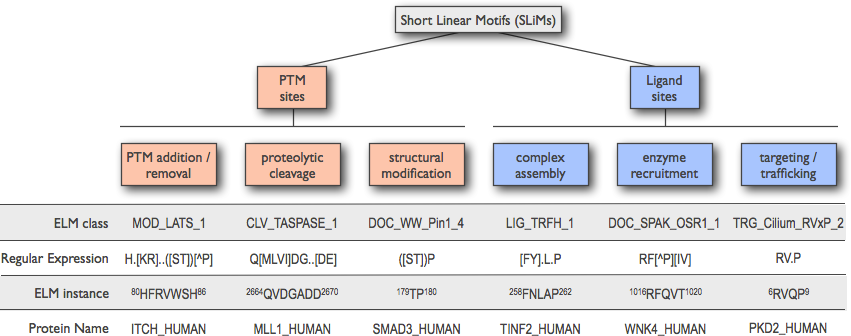
\includegraphics[width=\textwidth]{../Figures/functional_classification_of_SLiMs.png}
\textbf{Figure functional\_classification\_of\_SLiMs} For each ELM
class, the functional category to which it belongs is indicated by a
three-letter prefix. Each ELM class is defined by a regular expression.
Peptide sequences in proteins that match the regular expression of a
specific ELM class and that were experimentally validated to be
functional motifs are captured as ELM instances of that class. Degrons
are a specific subtype of enzyme-recruiting docking motifs (see text for
a detailed description).
\end{figure}

\section{Basic protocol 1: Explore the content of the ELM
DB}\label{basic-protocol-1-explore-the-content-of-the-elm-db}

The core of the ELM database is a repository of manually annotated
motifs and instances. As of December 2016, ELM contains over 260 motif
classes categorized into 6 different types: DOC (docking), LIG (Ligand
binding), DEG (degradation), CLV (cleavage), MOD (post translational
modifications), and TRG (targeting/anchoring) motifs (Figure
functional\_classification\_of\_SLiMs). These motifs are derived from
various types of experiments reported in literature. Each manually
annotated motif also has a set of bona fide instances (occurrences) of
this motif. Currently, there are over 3000 annotated instances annotated
from over 2500 publications. The motif classes and motif instances have
been uploaded by a large group of annotators from around the globe. The
complete catalogue of manually curated data can be searched, browsed and
explored on the ELM website

\subsection{Database content overview}\label{database-content-overview}

\begin{figure}[h!]
\centering
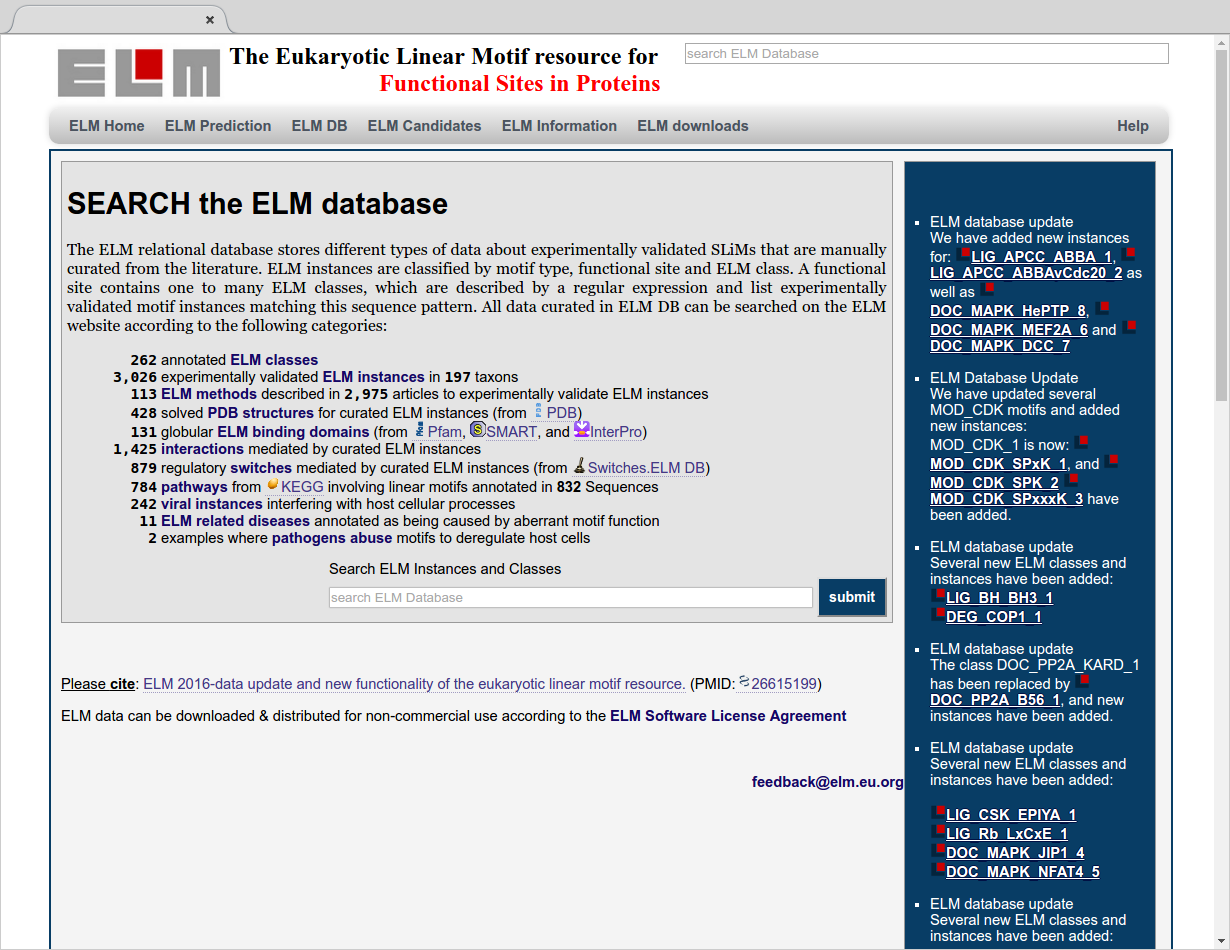
\includegraphics[width=\textwidth]{../Figures/TP53_2/stats.png} \textbf{Figure TP53-BP2-1}
The ELM database overview page (http://elm.eu.org/search.db).
\end{figure}

Step 1. Go to http://elm.eu.org and click on the tab ``ELM DB'' to
explore the content of the different types of data about experimentally
validated ELMs that were manually curated from the literature (Figure
TP53-BP2-1). This page contains a brief summary of the database content,
as well as the number of links to third-party databases. The table gives
an overview of the type and amount of information stored in the
database. Each line contains at least one link which will take you to
the corresponding contents page (eg. ``ELM instances'').

\begin{figure}[h!]
\centering
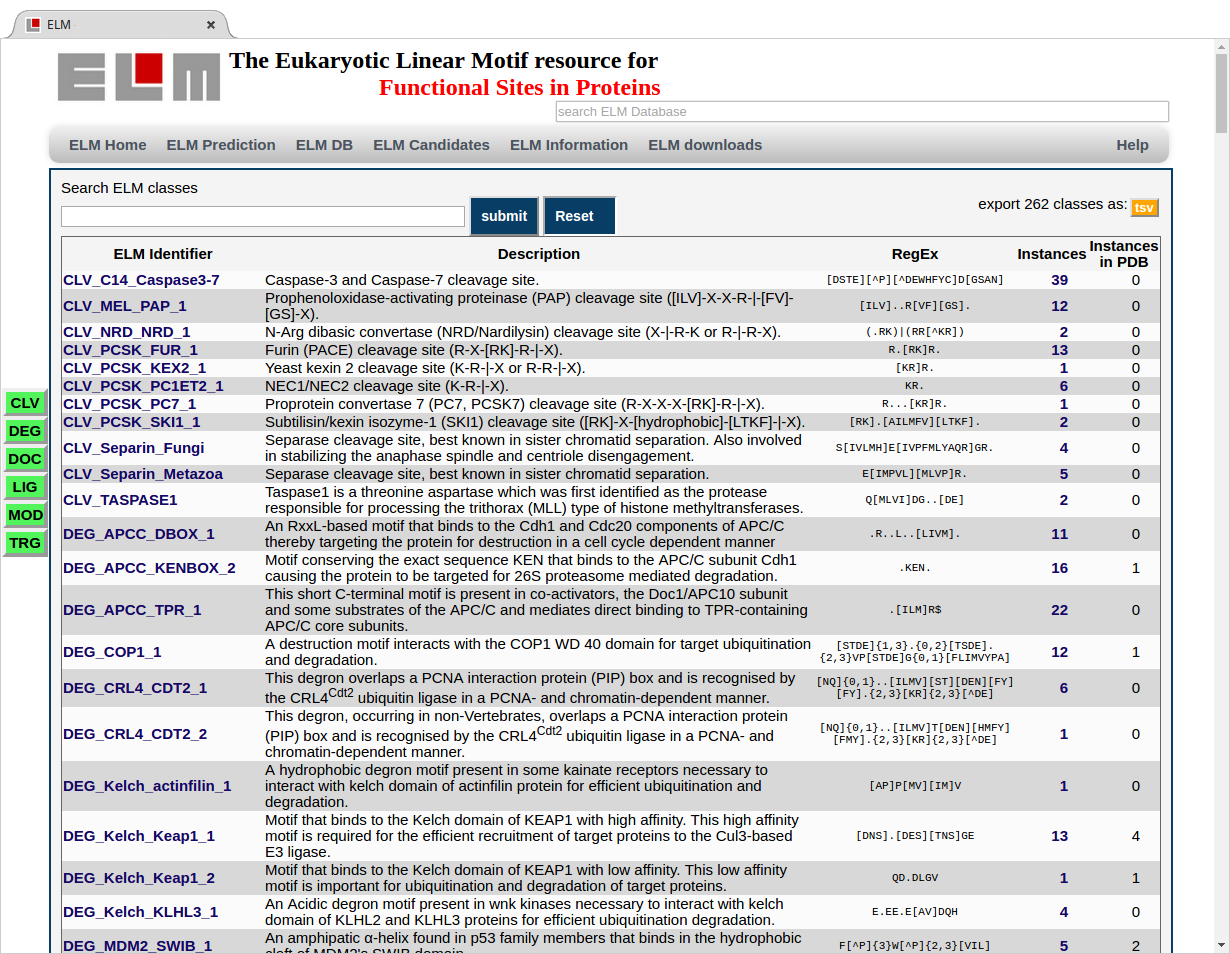
\includegraphics[width=\textwidth]{../Figures/TP53_2/elms.png} \textbf{Figure TP53-BP2-2}
The list of all motifs in the ELM database.
\end{figure}

Step 2. Click on the sub-menu ``ELM classes'' in ``ELM DB'' to see the
page with all of the ELM classes (Figure TP53-BP2-2). For each class,
the following information is provided: ELM identifier, short
description, regular expression, number of instances annotated for each
class, and number of structures available. For details on each class,
click on the ELM identifier; to get a list of annotated instances for an
individual class, click on the number of instances.

\begin{quote}
Use the search bar at the top of the page to filter for certain motif
classes. For example, typing ``MAPK'' and hitting submit will perform a
full-text search on all motif classes in the ELM database containing the
term ``MAPK''. The green buttons on the left can also be used to filter
this table. For example, toggling the ``DOC'' button will remove all
``DOC'' classes from the table (and clicking it again will bring them
back). Lastly, the yellow tsv link can be used to export all motif
classes as a ``tab separated values'' file.
\end{quote}

\begin{figure}[h!]
\centering
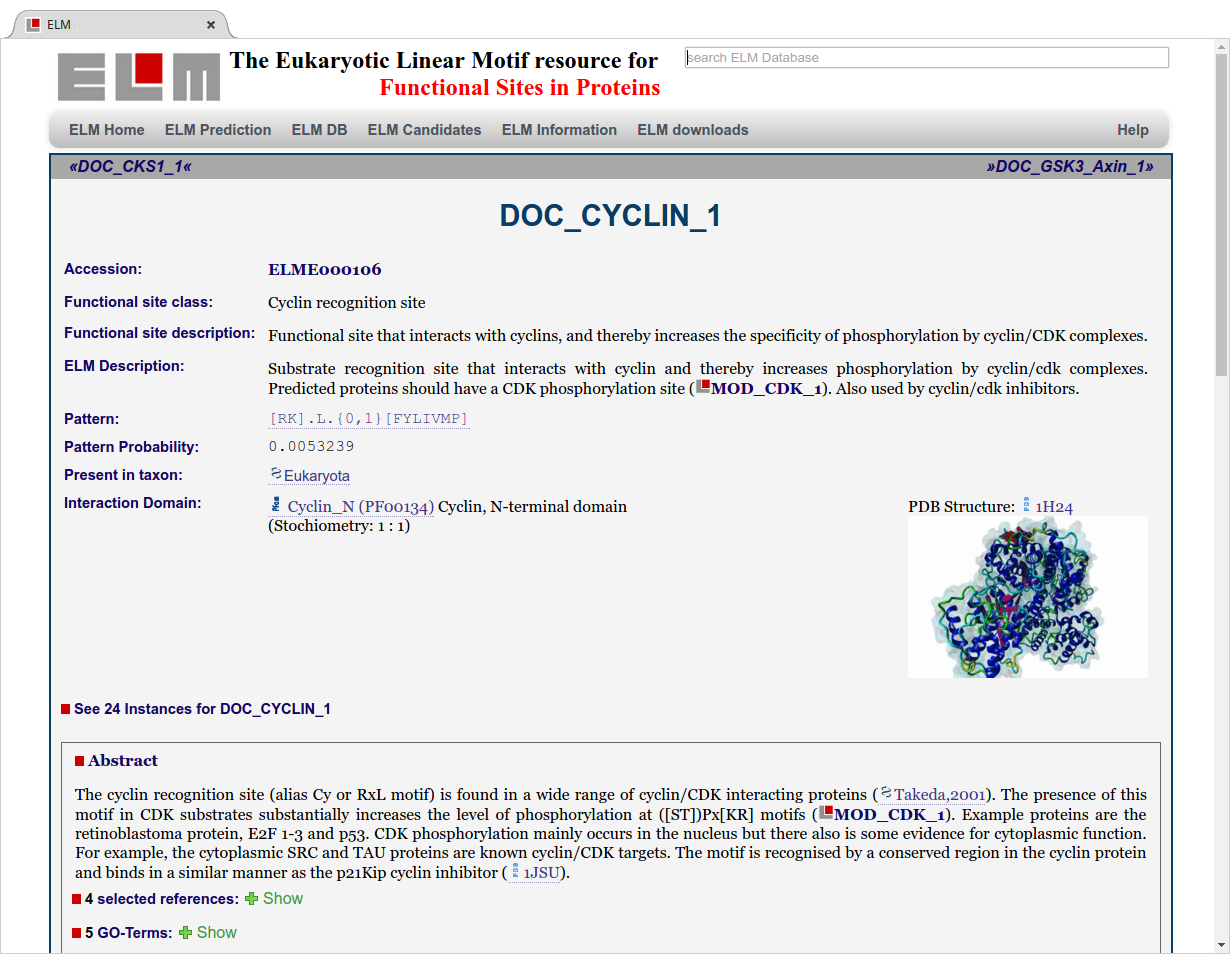
\includegraphics[width=\textwidth]{../Figures/TP53_1/doc_cyclin_1_class.png}
\textbf{Figure TP53-BP1- 4} The motif details page for
``DOC\_CYCLIN\_1''. This page contains all of the manual annotation
details for the DOC\_CYCLIN\_1 motif, the biological background
summarized from the scientific literature including links to the primary
literature and to external resources (Pubmed (\cite{27899561}),
GeneOntology (\cite{27899567}), PDB (\cite{12037327}) and more).
\end{figure}

Step 3. Search the table for the term ``DOC\_CYCLIN\_1'' and click on
its link to navigate to the page with details about the
``DOC\_CYCLIN\_1'' motif class (Fig TP53-BP1-4). This page contains a
description of the functional site class (a Cyclin recognition site),
and a short description of the ELM and its regular expression, as well
as a probability score, the taxonomic distribution of the motif and
which domain (if any) is responsible for the interaction.

\begin{quote}
The probability score is the probability that the regular expression
represents a random selection of amino acids (similar to an information
content score). A lower score indicates that the motif pattern is more
difficult to find by chance in a random sequence.
\end{quote}

Step 4. Scroll further down the ``DOC\_CYCLIN\_1'' page (Fig TP53-BP1-5)
to view more details about the manually annotated data and instances in
the database (to the text box starting with the ``Abstract''). The
``abstract'' contains a more detailed description of the motif
annotation. Click on the ``Show'' button next to the ``selected
references'' header for a list of publications relevant to this motif.
Click on ``Show'' next to ``GO terms'' for a complete list of all GO
terms annotated for this motif.

Step 5. Scroll further down the ``DOC\_CYCLIN\_1'' page (Fig TP53-BP1-5)
to view the ``Instances'' header. This table contains the list of all
annotated instances in the database of this motif. This includes the
protein identifier, the start and end positions of the instance, the
specific sequence matching the regular expression and the logic of the
instance. The ``\# Ev.'' indicates the number of experimental evidences
associated with the annotation (see section XXX below). Organism is the
species in which the protein is found. Lastly the ``Notes'' column
contains links to any ``interactions'' or ``switches'' present in the
database, as well as links to PDB if this structure exists in PDB.

\subsubsection{Browsing annotated
instances}\label{browsing-annotated-instances}

\begin{figure}[h!]
\centering
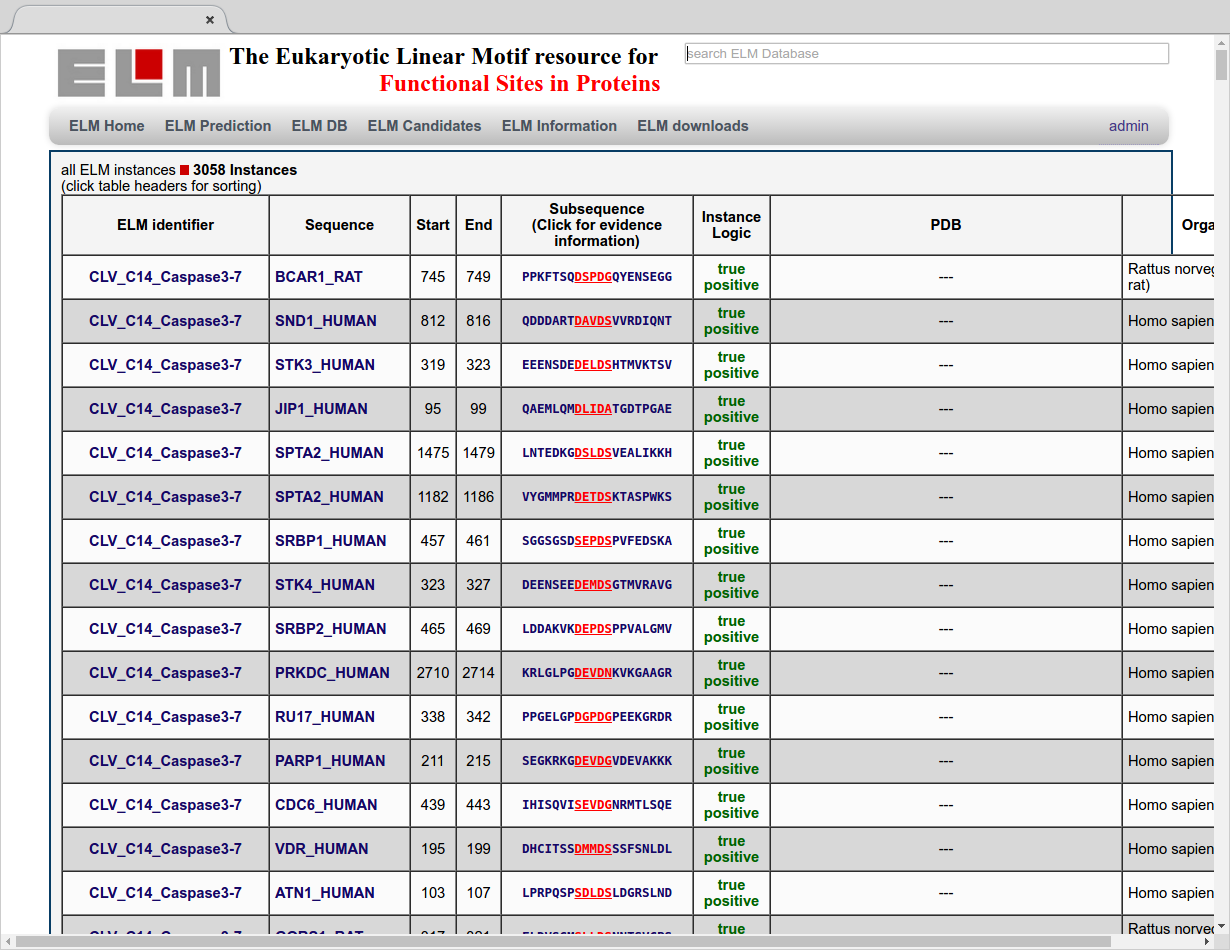
\includegraphics[width=\textwidth]{../Figures/TP53_2/instances.png} \textbf{Figure
TP53-BP2-3} The list of all instances in the ELM database.
\end{figure}

Step 6. Click on the sub-menu ``ELM instances'' in ``ELM DB'' to go to
the page which lists all of the instances in the database (Figure
TP53-BP2-3). This table contains a list of all instances in the
database.

\begin{quote}
Use the search filters at the top of the page to limit the results by a
full text search, by instance logic, or organisms. Similar to the ELM
classes page (previous step) these results can be filtered by motif
class using the green toggle filters on the left hand side. Lastly, the
yellow buttons at the top of the page can be used to download the
instances in the following formats: gff, pir, fasta or tsv.
\end{quote}

\begin{figure}[h!]
\centering
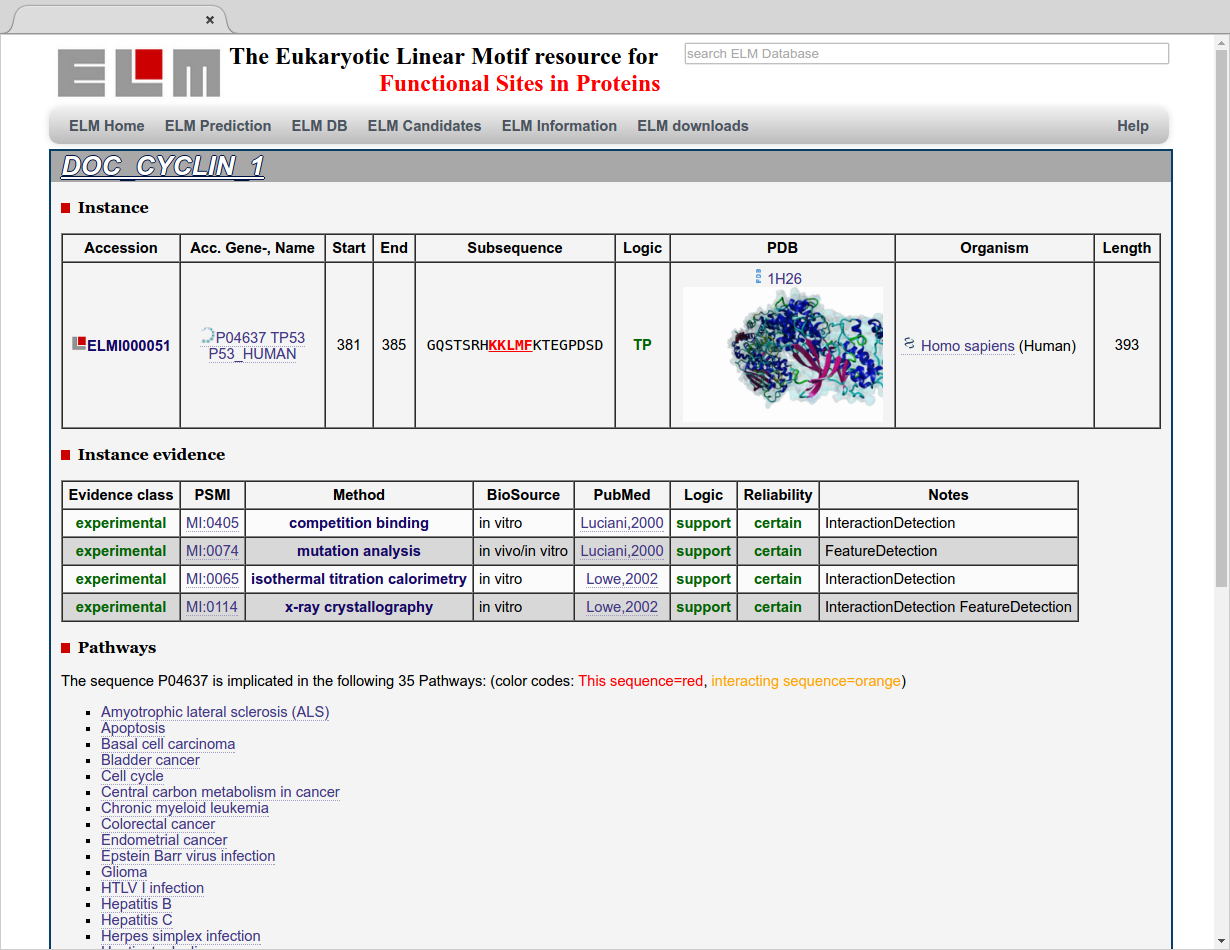
\includegraphics[width=\textwidth]{../Figures/TP53_1/doc_cyclin_1_instance.png}
\textbf{Figure TP53-BP1- 5} The instance details page for the
``DOC\_CYCLIN\_1'' instance annotated for protein P53\_HUMAN with
start/end position ``381-385''. This page also contains links to many
external databases including Uniprot (\cite{25348405}), PDB
(\cite{12037327}), NCBI taxonomy, Pubmed (\cite{27899561}), and KEGG
Pathways (\cite{26476454}), as well as the PSI-MI controlled vocabulary
(\cite{17925023}).
\end{figure}

Step 7. Type ``p53\_human'' in the search box to search for ELM
Instances in this protein. Find the row for the ELM class
``DOC\_CYCLIN\_1'' and click on the startposition ``381'' to go to the
instance details page of this instance. The top part of the page
contains details about the instance and the protein it was identified
in.

Step 8. Scroll down to the ``Instance Evidence'' header to view details
on the experimental evidence used to annotate this instance. This table
also contains the ``evidence class'', and descriptions of the methods
used from PSI-MI (\cite{17925023}) as well as the Literature references
in which the experiments were published.

\begin{quote}
(Here we should explain what ``evidence class'', ``biosource'',
``Logic'', ``Reliability'' and ``Notes'' actually mean).
\end{quote}

\subsection{Details on molecular switches, motif-mediated pathways and
other external
resources.}\label{details-on-molecular-switches-motif-mediated-pathways-and-other-external-resources.}

Step 9. Scroll further down to the header ``Pathways'' to view pathway
information. This is a list of all of the pathways in which the protein
p53 is known to be involved (according to KEGG). Click on a pathway to
see the localization of p53 in the corresponding KEGG pathway.

\begin{figure}[h!]
\centering
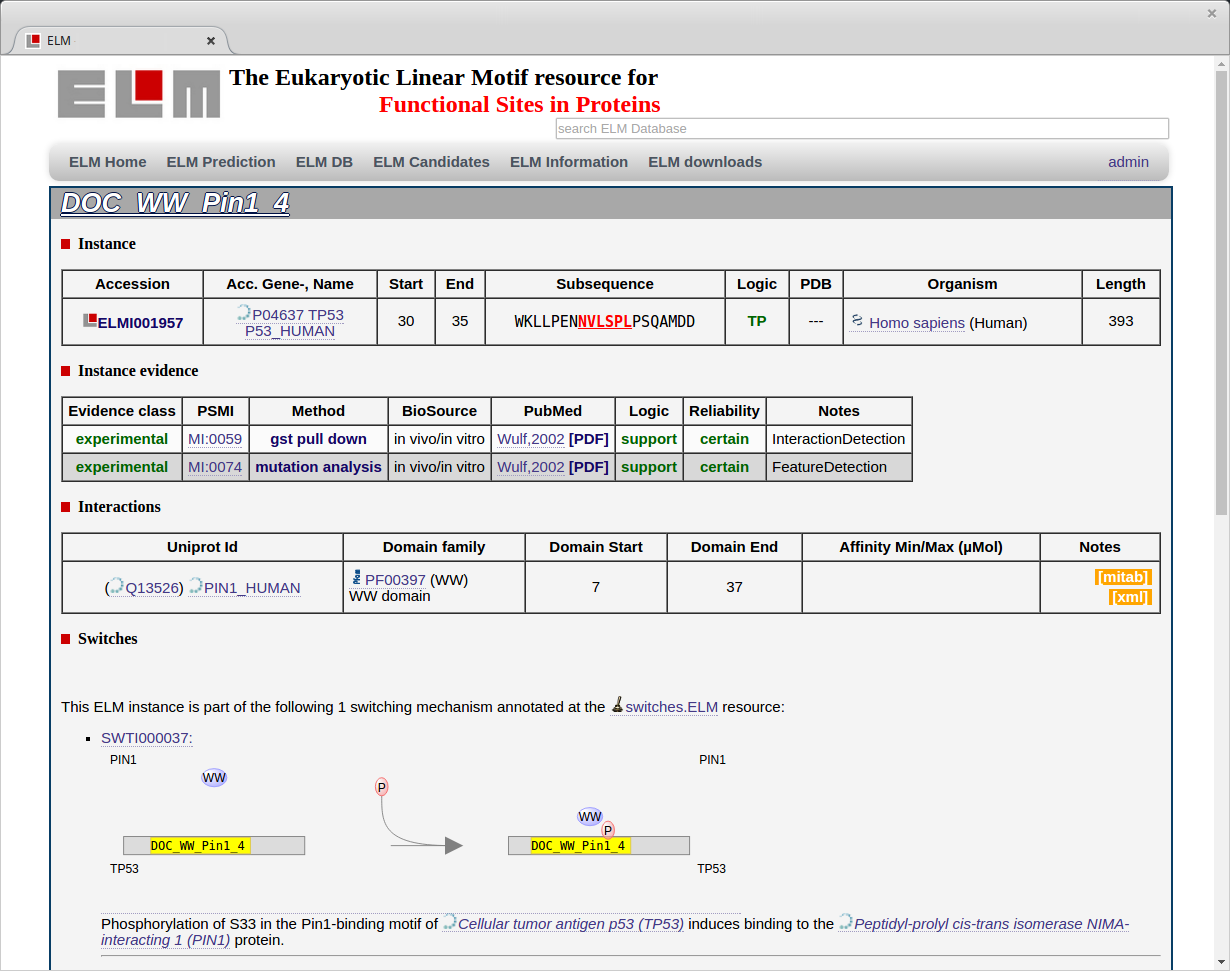
\includegraphics[width=\textwidth]{../Figures/TP53_1/doc_ww_pin_1_4_instance.png}
\textbf{Figure TP53-BP1-6} The instance details page for the
``DOC\_WW\_Pin1\_4'' instance found in P53 with start/end position
``30-35''.
\end{figure}

Step 10. Repeat the previous search by clicking on the sub-menu ``ELM
instances'' in ``ELM DB'' and type ``p53\_human'' in the search box.
This time, try to find the ELM instance ``DOC\_WW\_Pin1\_4'' motif with
the start/end position ``30-35'' (You can sort the table by clicking on
the header lines eg. on ``Start'' to sort by startposition ). Click on
the start/endposition or the subsequence which will take you to the
details page as shown in Fig TP53-BP1-6. This page is similar to that
described for the P53 instance ``DOC\_CYCLIN\_1'' (Fig TP53-BP1-5);
additionally, for this instance there is information available about its
interaction partner and a molecular switch which is mediated by this
motif instance.

Step 11. Scroll down to the ``Interactions'' header to view information
about this instance's interactions (Fig TP53-BP1-6). This instance
interacts with PIN1\_Human via the ``WW'' domain (PFAM identifier
PF00397; found on position 7--37 in PIN1\_Human). If available, binding
affinities are also shown here. Interaction data is made available in
Mitab and xml format (\cite{17925023}).

Step 12. Scroll further down to the ``Switches'' section for a brief
overview of the switches details of this instance obtained form
``switches.ELM'' (\cite{23550212}) (Fig TP53-BP1-6). This particular
instance is involved in the switch phosphorylating P53. Clicking on the
diagram will open an external link to the ``switches.ELM'' website.

\begin{figure}[h!]
\centering
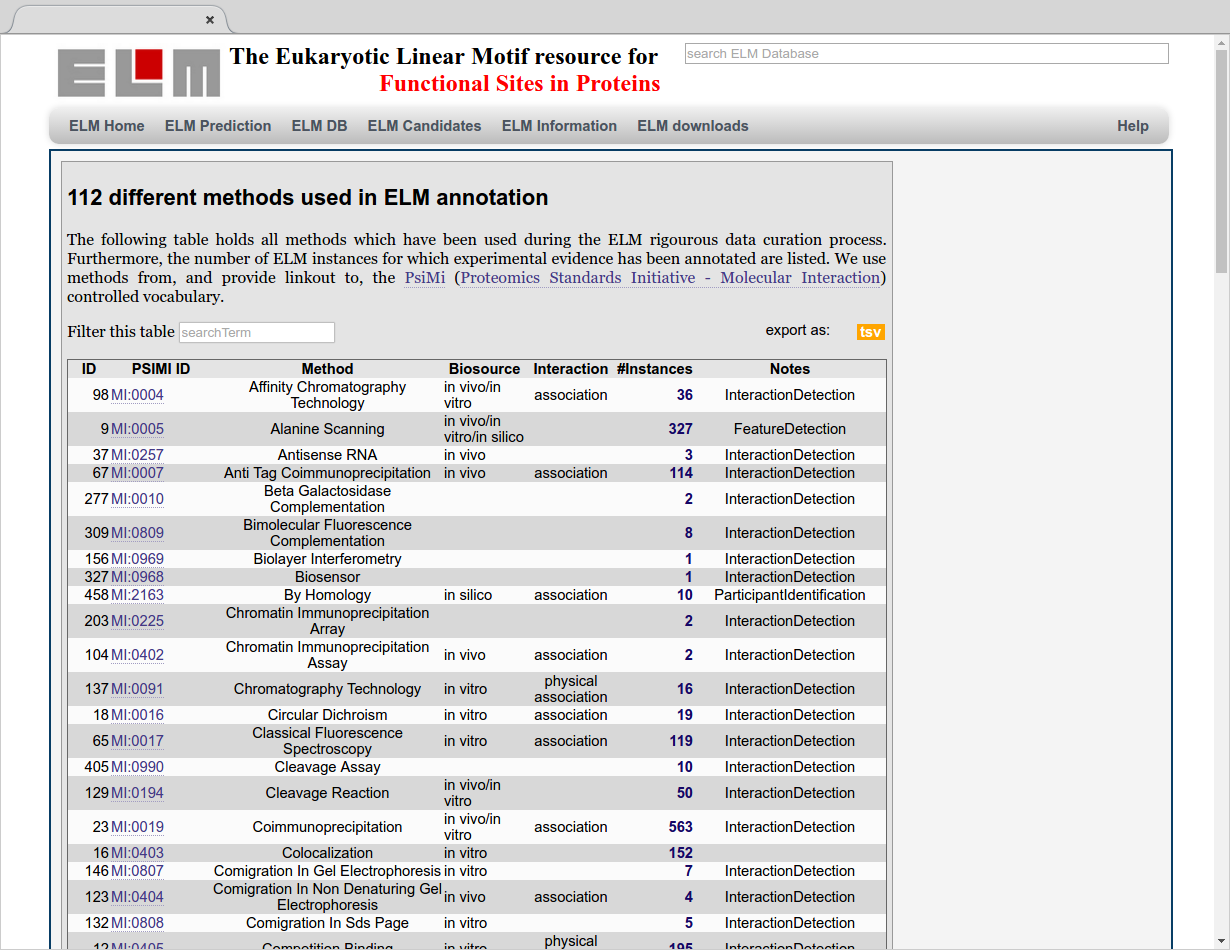
\includegraphics[width=\textwidth]{../Figures/TP53_2/methods.png} \textbf{Figure
TP53-BP2-4} The list of all experimental methods used in the ELM
database.

Step 13. Click on the sub-menu ``ELM methods'' in ``ELM DB'' to see a
list of all experimental methods which have been used to identify motifs
and instances (figure TP32-BP2-4). This table shows the internal method
identifier in the first column, a link to the corresponding entry in the
PSI-MI database (\cite{17925023}), and the method name as annotated by
the PSI-MI controlled vocabulary, as well as the type of experiment (in
vitro/in vivo). Clicking on the link in the ``instances'' column will
list all instances annotated using that method.
\end{figure}

\begin{quote}
The filter bar on the top page can be used to filter the list of
methods. The \emph{tsv} link creates a downloadable file in ``tab
separated values'' format.
\end{quote}

\begin{figure}[h!]
\centering
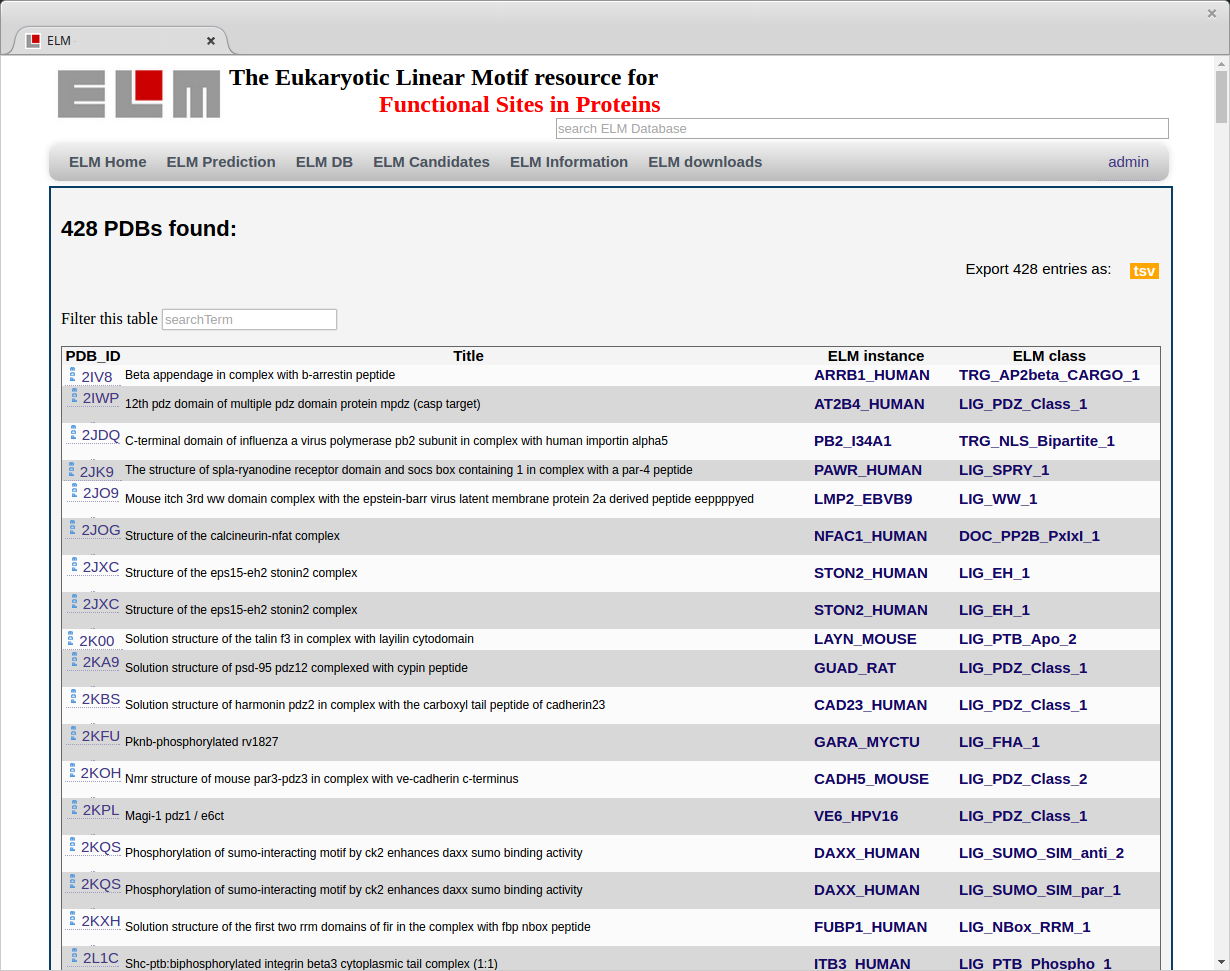
\includegraphics[width=\textwidth]{../Figures/TP53_2/pdbs.png} \textbf{Figure TP53-BP2-5}
The list of all known structures in PDB also in ELM.
\end{figure}

Step 14. Click on the sub-menu ``ELM pdb structures'' in ``ELM DB'' to
see a list of all macromolecular structures in the ELM database (Figure
TP53-BP2-5). Structures annotated in ELM ideally (but not always) show
both interaction partners, motif and domain. This page also contains
links to RCSB (\cite{12037327}), the individual instance and the motif
class of that instance.

\begin{quote}
The filter bar on the top page can be used to filter the list of
structures shown . The \emph{tsv} link creates a downloadable file in
``tab separated values'' format. The \emph{tsv} file contains the PDB
id, uniprot name, and ELM class.
\end{quote}

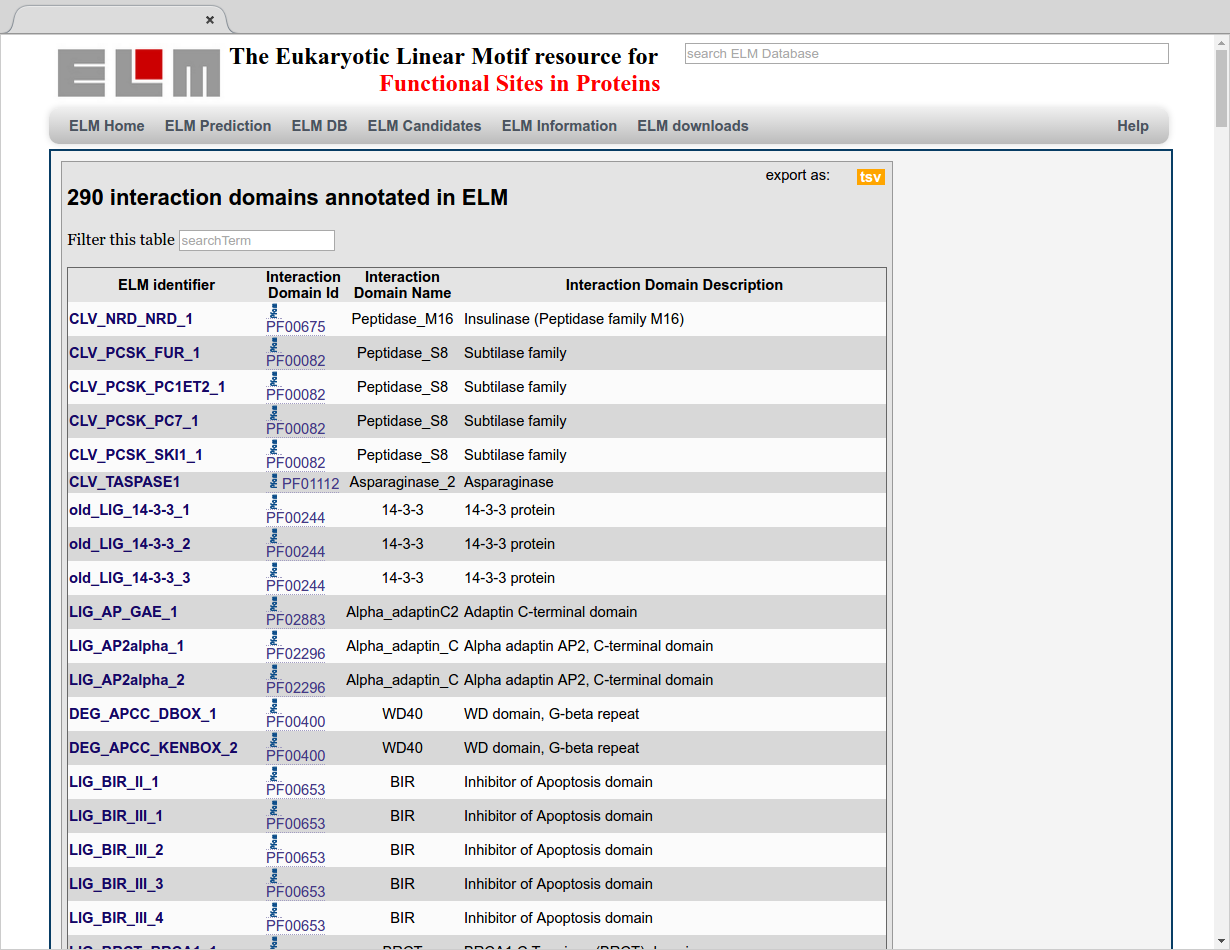
\includegraphics[width=\textwidth]{../Figures/TP53_2/interactiondomains.png}
\textbf{Figure TP53-BP2-6} A list of all interactions annotated in the
database.

Step 15. Click on the sub-menu ``ELM binding domains'' in ``ELM DB'' to
see a complete list of all the interaction domains in ELM (Figure
TP53-BP2-6). This table shows the ELM classes which have been annotated
with a corresponding interaction domain. This table shows the ELM class,
a link to the Pfam (\cite{26673716}) / SMART (\cite{25300481}) /
InterPro (\cite{27899635}) domain, as well as the name of the
interacting domain followed by a brief description.

\begin{quote}
The filter bar on the top page can be used to filter the list of
interactions shown. The \emph{tsv} link creates a downloadable file in
``tab separated values'' format.
\end{quote}

\subsection{Links to external
resources}\label{links-to-external-resources}

\begin{figure}[h!]
\centering
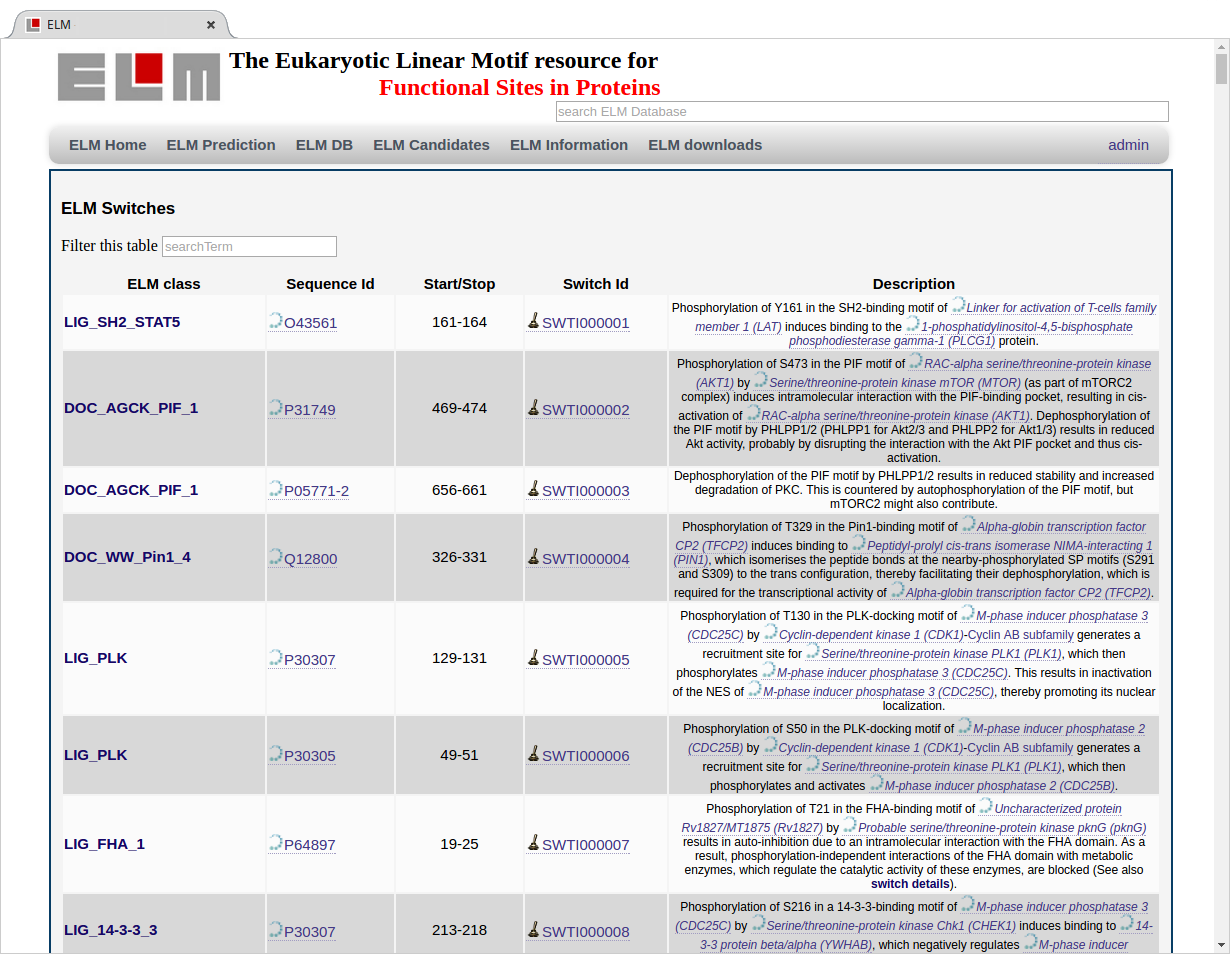
\includegraphics[width=\textwidth]{../Figures/TP53_2/switches.png} \textbf{Figure
TP53-BP2-7} A list of all switches annotated in ELM.
\end{figure}

Step 16. Click on the sub-menu ``ELM switches'' in ``ELM DB'' to see a
complete list of all the switches in ELM (Figure TP53-BP2-7). This table
shows the motif class, contains a link to Uniprot, and the start and
stop positions of the motif mediating the switch. The last two columns
have links to switches.ELM, and a brief description of the switch also
taken from switches.ELM (\cite{23550212}).

\begin{quote}
The filter bar on the top page can be used to quickly filter the list of
interactions shown.
\end{quote}

\subsection{Exploring KEGG pathways from
ELM}\label{exploring-kegg-pathways-from-elm}

\begin{figure}[h!]
\centering
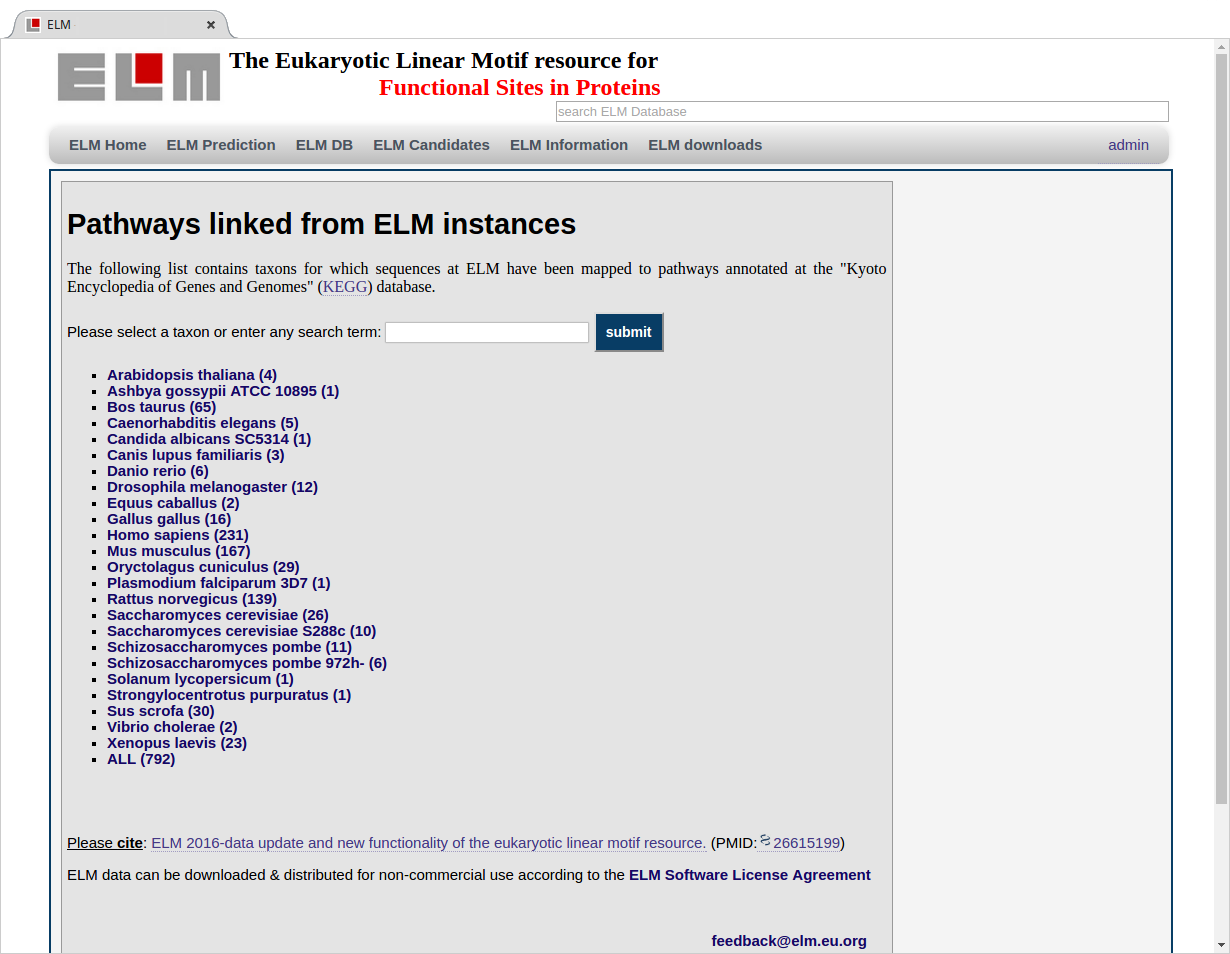
\includegraphics[width=\textwidth]{../Figures/TP53_2/pathways.png} \textbf{Figure
TP53-BP2-9} A list of all Pathways from KEGG with proteins in ELM.
\end{figure}

Step 17. Click on the sub-menu ``ELM pathways'' in ``ELM DB'' to see a
list of all pathways contained in ELM (Fig. TP53-BP2-9). Pathways are
from the ``Kyoto Encyclopedia of Genes and Genomes'' (KEGG
\cite{26476454}) database mapped to ELM instances. Click on a species
(for example ``Homo sapiens'') for a complete list of all Human pathways
which have a protein annotated in ELM, and links to the pathways on
KEGG.

\begin{figure}[h!]
\centering
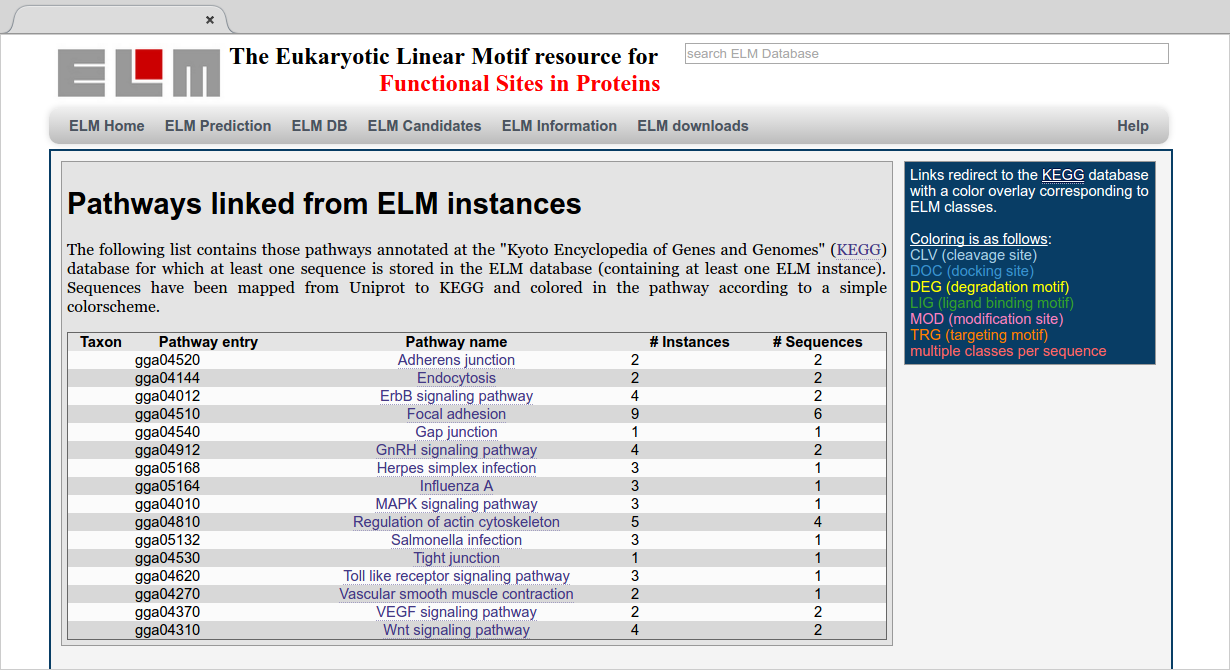
\includegraphics[width=\textwidth]{../Figures/TP53_2/pathways_example.png} \textbf{Figure
TP53-BP2-10} A list of all pathways in Gallus Gallus

Step 18. On the ``ELM pathways'' page (Fig. TP53-BP2-9) click on the
link ``gallus gallus'' to navigate to the page containing all pathways
annotated for chicken. This page contains links to all KEGG pathways for
the taxon \emph{gallus gallus} with annotated instances in the ELM
database.
\end{figure}

\begin{figure}[h!]
\centering
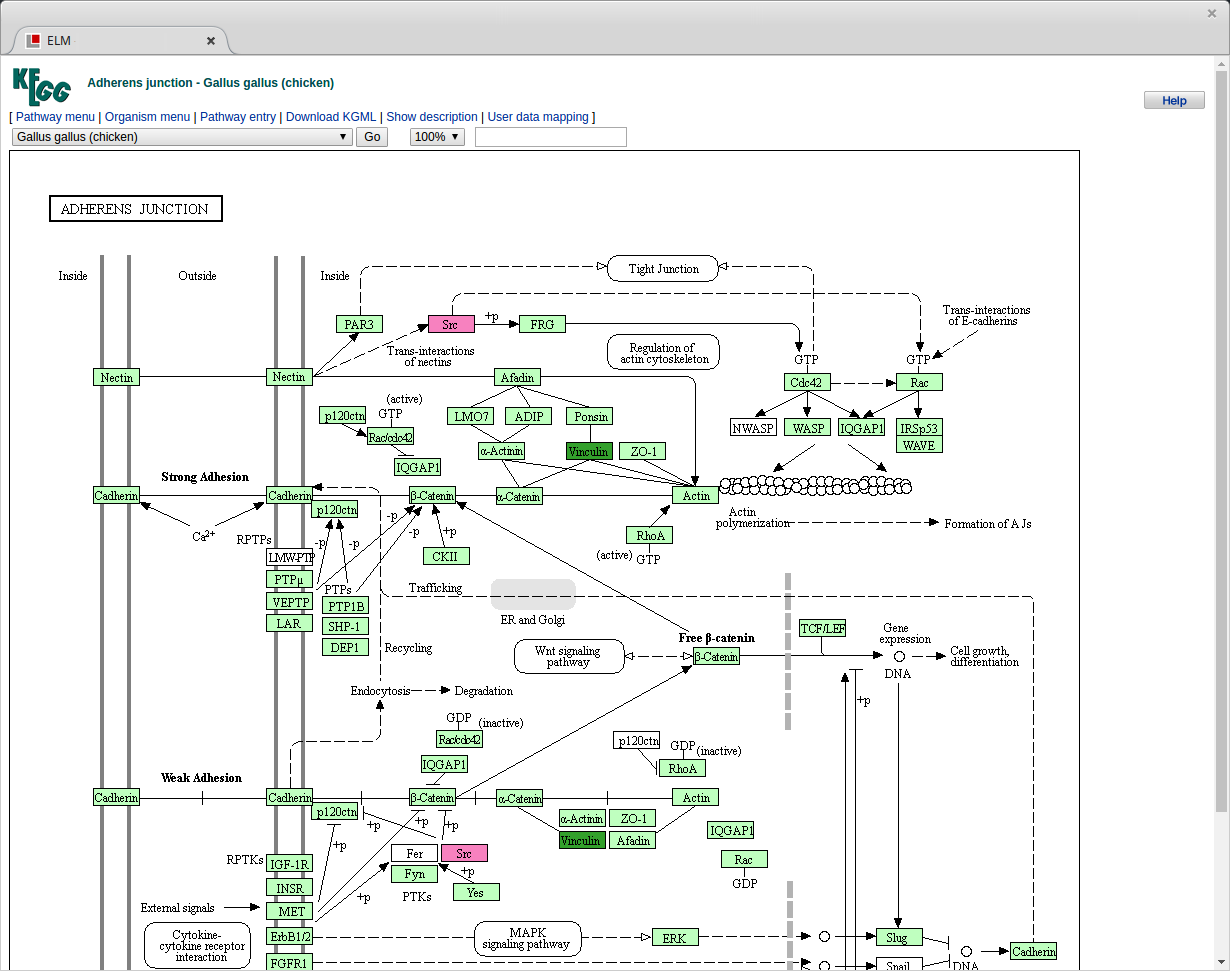
\includegraphics[width=\textwidth]{../Figures/TP53_2/pathways_kegg.png} \textbf{Figure
TP53-BP2-11} A list of all annotated pathways for taxon \emph{gallus
gallus}
\end{figure}

Step 19. One the page with chicken pathways (Fig. TP53-BP2-10) click on
``Adherens junction'' to the KEGG entry for this pathway, with proteins
color overlay corresponding to ELM classes (see the color legend right
side of figure TP53-BP2-10).

\subsection{Infections and Diseases}\label{infections-and-diseases}

\begin{figure}[h!]
\centering
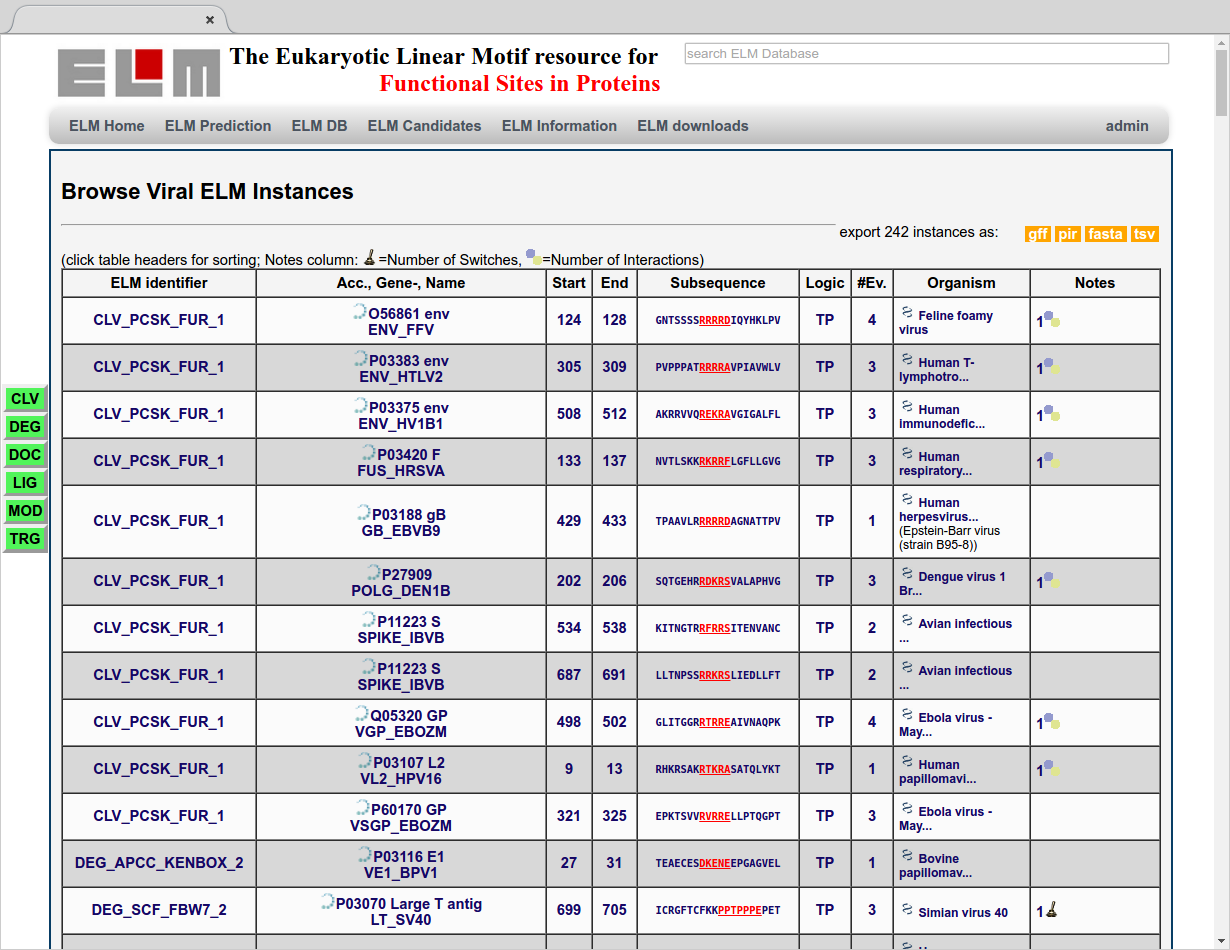
\includegraphics[width=\textwidth]{../Figures/TP53_2/viruses.png} \textbf{Figure
TP53-BP2-11} A Table of the ELM instance abused by viruses

Step 20. Click on the sub-menu ``ELM virus instances'' in ``ELM DB'' to
see a list of all instances in ELM that have been annotated as being
abused by viruses (Fig TP53-BP2-9). The columns are identical to those
listed in section XXX step YYY (Figure ZZZZ).

\begin{quote}
The green buttons on the left can be used to filter this table by motif
class. Click on the yellow links on the top right of the page to
download the (complete) table in gff, pir, fasta or tsv format. (See
section XXX for a description of these formats.)
\end{quote}

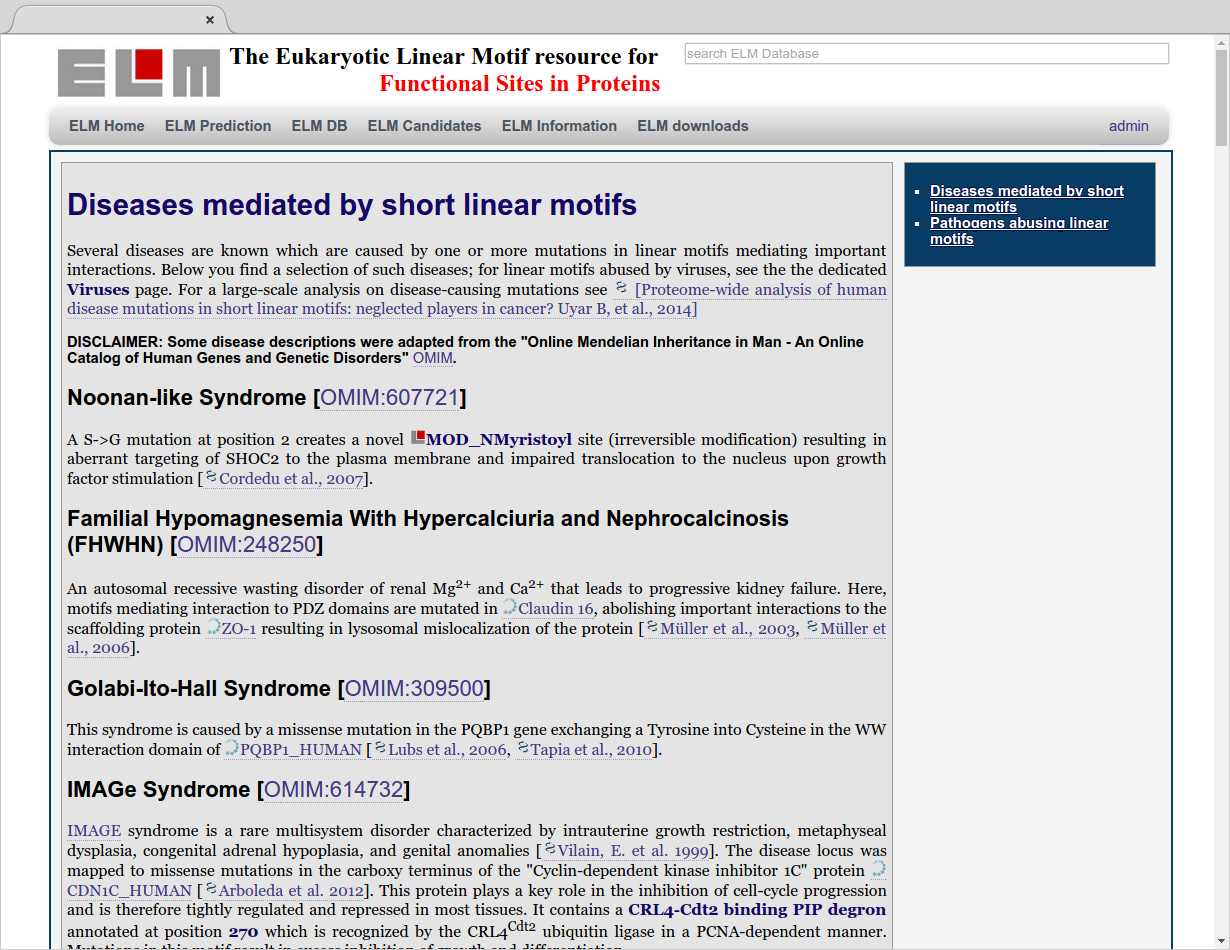
\includegraphics[width=\textwidth]{../Figures/TP53_2/diseases.png} \textbf{Figure
TP53-BP2-8} A list of all diseases in ELM.

Step 21. Click on the sub-menu ``ELM diseases'' in ``ELM DB'' to see a
list of all motif classes that have been annotated with a disease.
Disease information is taken from the OMIM database.

\begin{quote}
This table also includes the diseases found under the ``ELM pathogenic
abuse'' menu in ``ELM DB''. (right?)
\end{quote}

\section{Alternate protocol 2: General Search
Box}\label{alternate-protocol-2-general-search-box}

A general search text box is available to explore the manually curated
information in the ELM DB. This is a ``Full-text'' search which is
performed on selected columns of the database therefore some attention
(better term?) should be applied when evaluating the retrieved results.

\begin{figure}[h!]
\centering
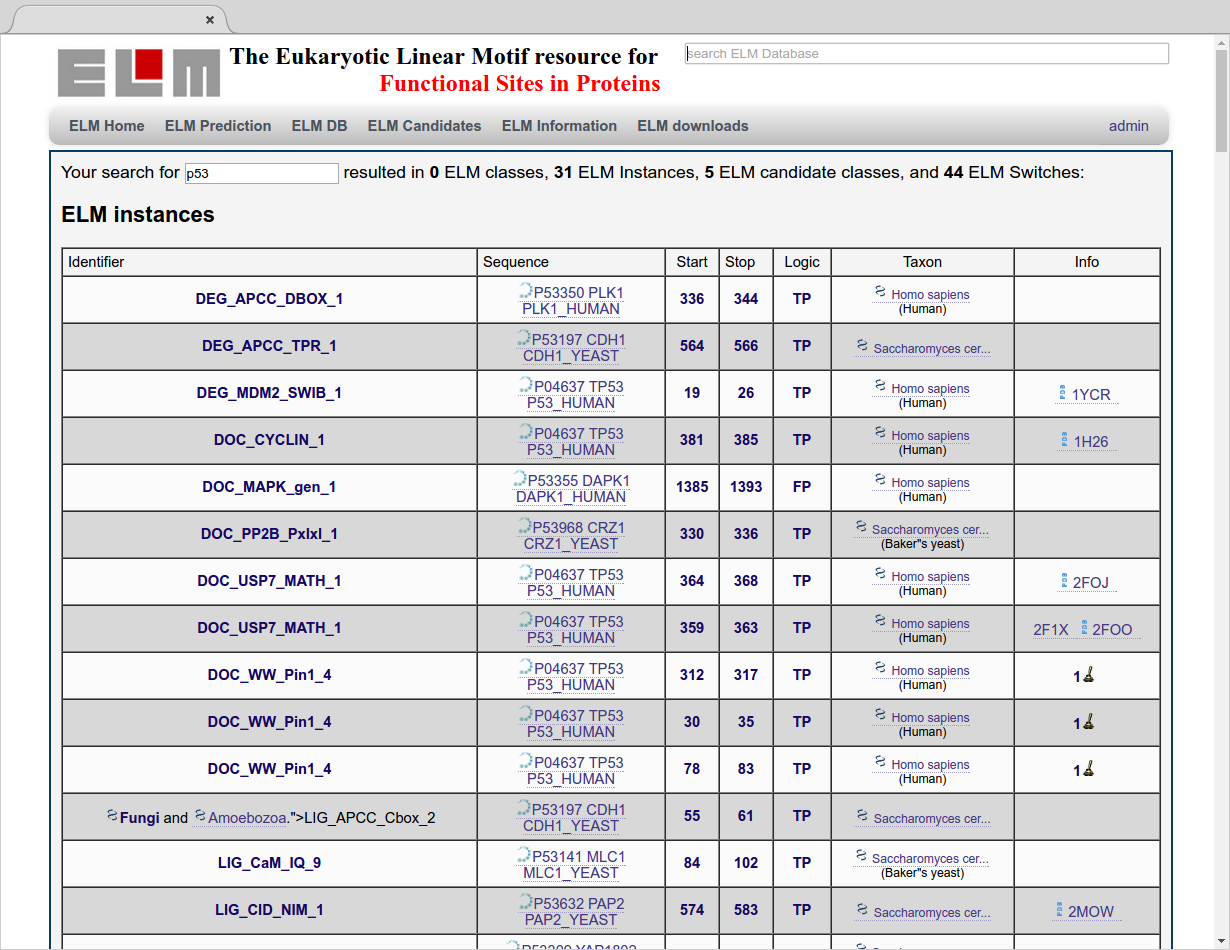
\includegraphics[width=\textwidth]{../Figures/TP53_3/TP53_instances.png} \textbf{Figure TP53-AP1-1}
@e

\begin{figure}[h!]
\centering
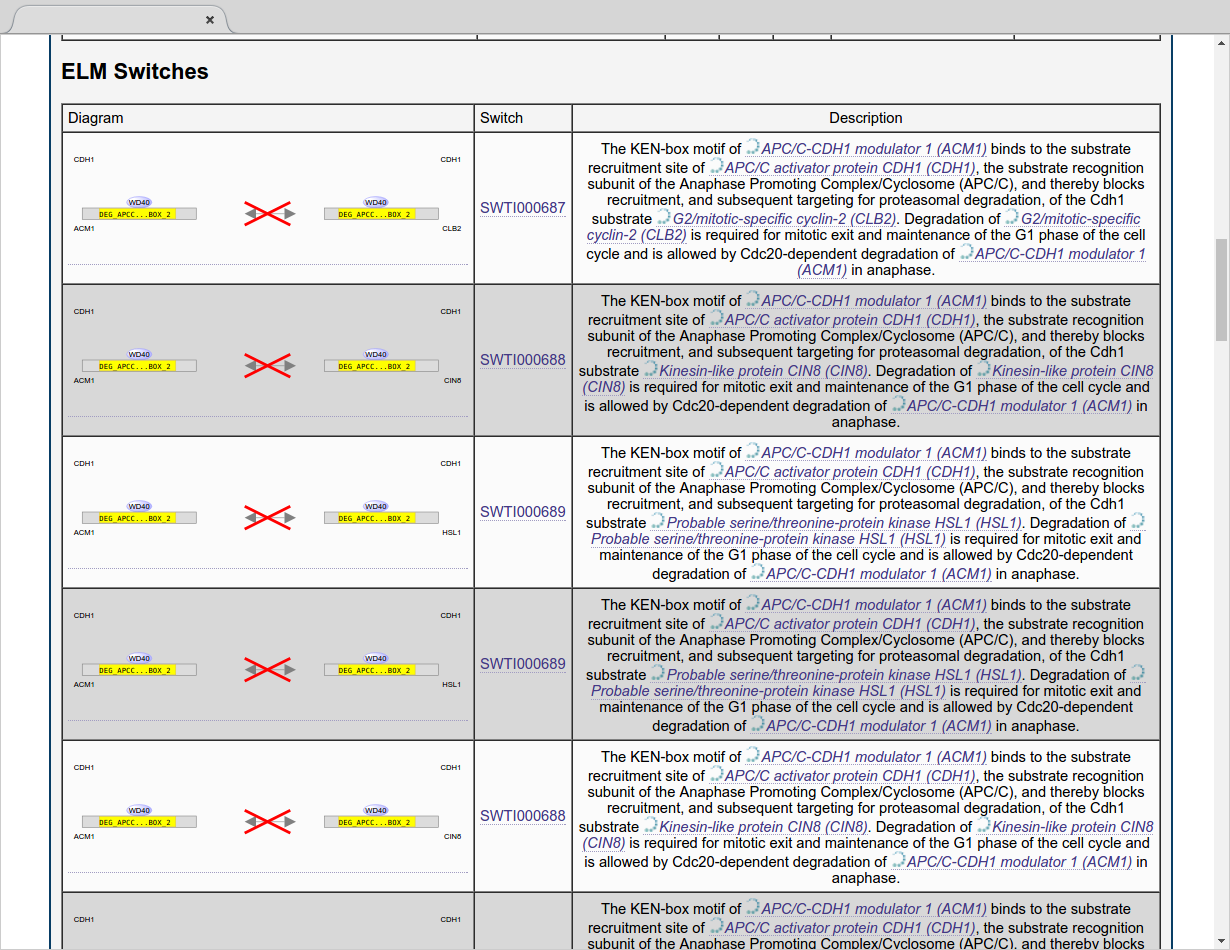
\includegraphics[width=\textwidth]{../Figures/TP53_3/TP53_switches.png} \textbf{Figure
TP53-AP1-2}

\end{figure}

\begin{figure}[h!]
\centering
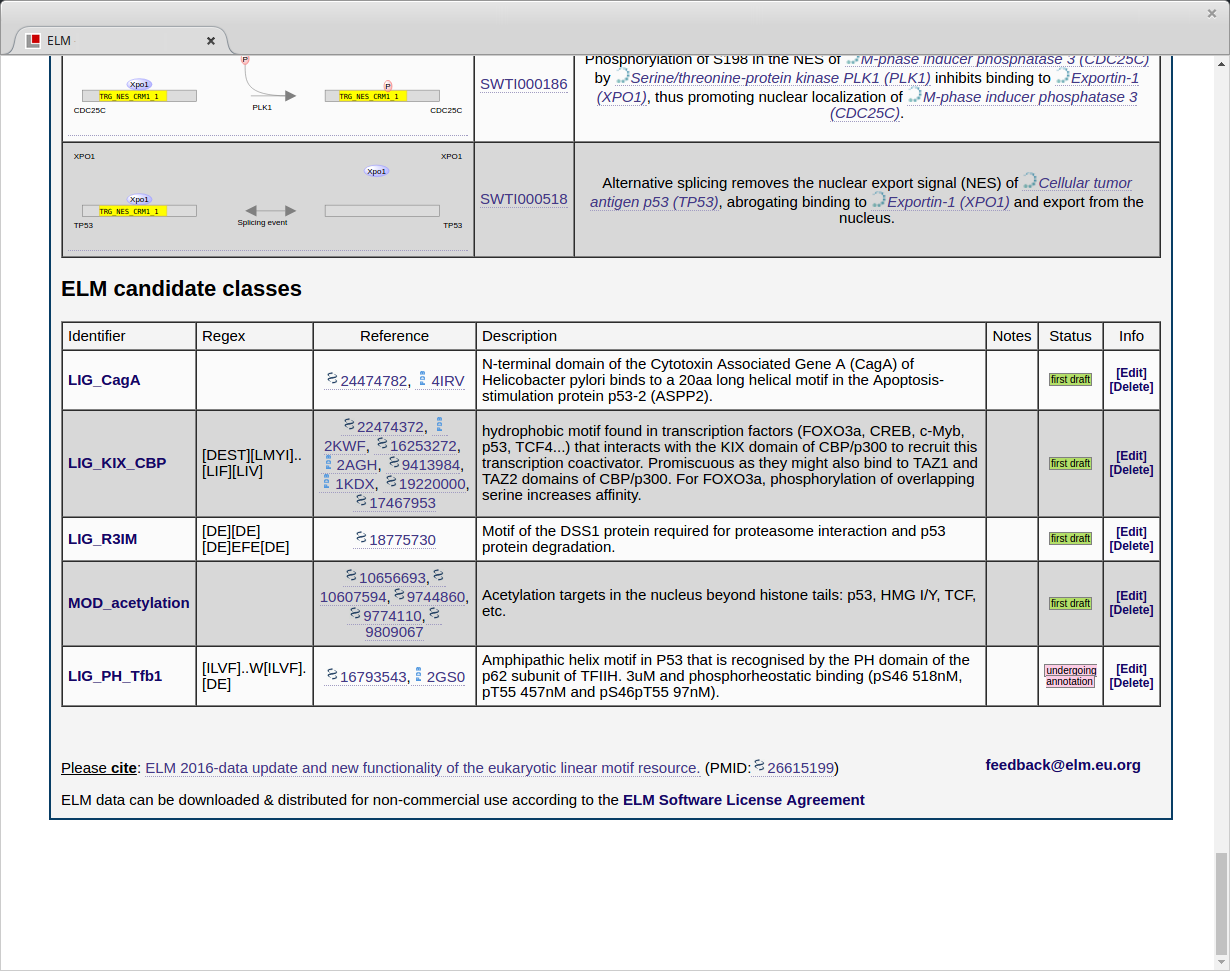
\includegraphics[width=\textwidth]{../Figures/TP53_3/TP53_candidates.png} \textbf{Figure
TP53-AP1-3}
\end{figure}

Example 1: perform a search using the keyword `p53'. The results are
retrieved in the following section: ELM instances (xx matches), ELM
Switch (xx matches), and ELM Candidate classes (xx matches). One will
find proteins such as CDH1\_YEAST (because of its accession P53197)
which may or may not be what one wants.

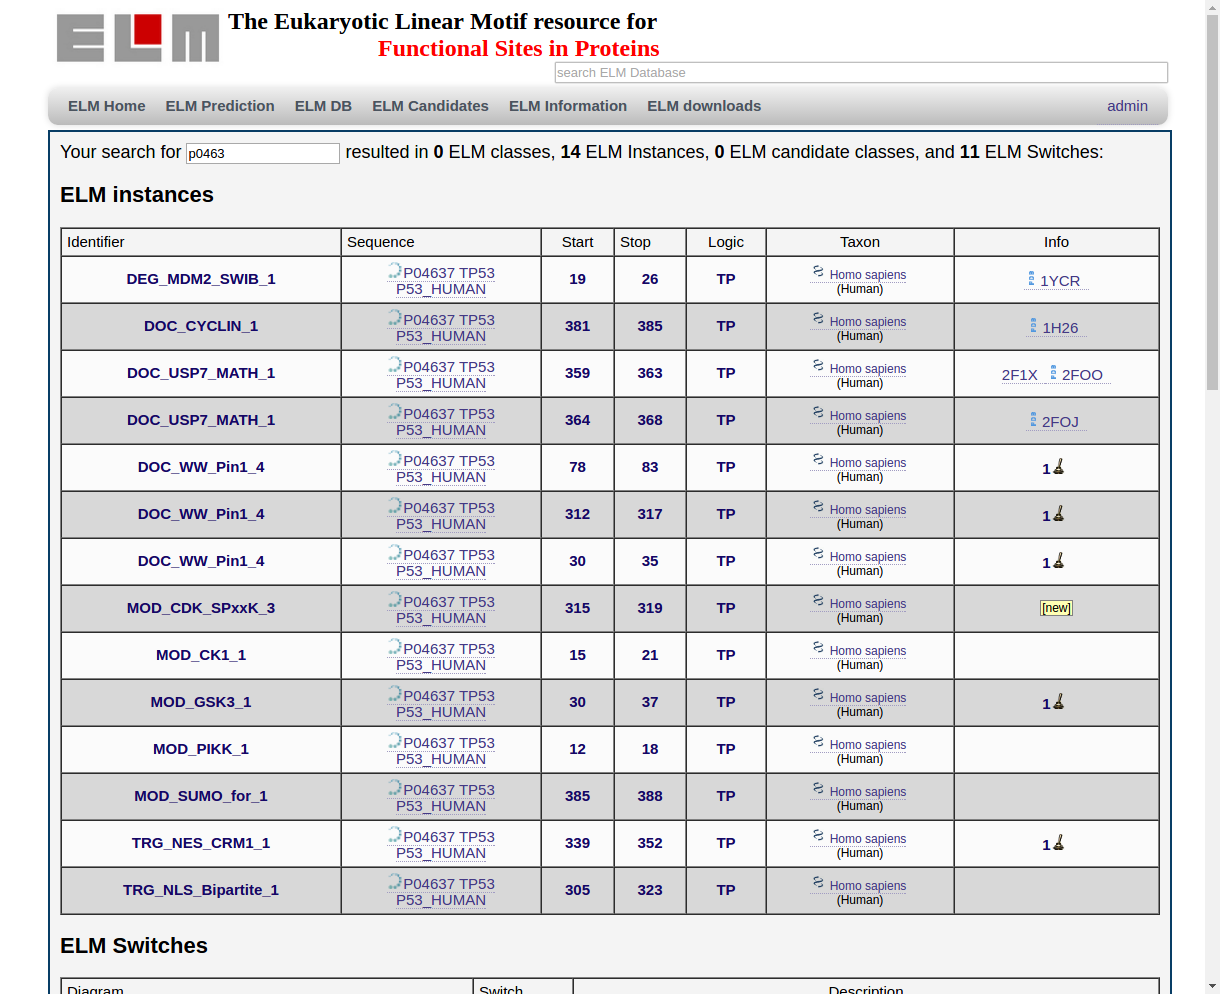
\includegraphics[width=\textwidth]{../Figures/TP53_3/P04637_instances.png} \textbf{Figure
TP53-AP1-4}

Example 2: perform a search using the gene id TP53 or the UniProt Acc
P04637. The results are retrieved in the following section: ELM
instances (xx matches), ELM Switch (xx matches). The retrieved hits are
less, but more specific compared with the search with `53'. However,
there are no matches in ELM Candidate classes tough some content is
related to the p53 protein.

\section{Basic Protocol 2: Predicting ELMs in
sequences}\label{basic-protocol-2-predicting-elms-in-sequences}

One of the most useful (and used) features in ELM is the ability to
detect motifs in proteins and sequences. Given a protein's amino acid
sequence, the ``EML Predictions'' pipeline searches for occurrences of
each motif class using regular expressions, apply a set of filters to
help judging results, and to visualize resulting set of putative motifs.

In this protocol we will be viewing the manually annotated data of a
typical protein, using p53 (Uniprot ID: P53\_HUMAN/P04637) as an
example. We will cover how to find the manually annotated motifs and
instances, and how to find the motif instances, the references used to
annotate each instance, the experimental protocols used, and additional
information including relationships to biological pathways (such as KEGG
\cite{26476454}), diseases (from OMIM \cite{17357067}) and molecular
switches (in switches.ELM \cite{23550212}).

\subsection{Necessary Resources}\label{necessary-resources}

\subsubsection{Software \& Hardware}\label{software-hardware}

A modern browser such as Firefox, Chrome, or Safari. ELM is best viewed
on a laptop or desktop computer, although tablets and smartphones will
also work.

\subsection{Predicting ELM instances using data from ELM
database}\label{predicting-elm-instances-using-data-from-elm-database}

\begin{figure}[h!]
\centering
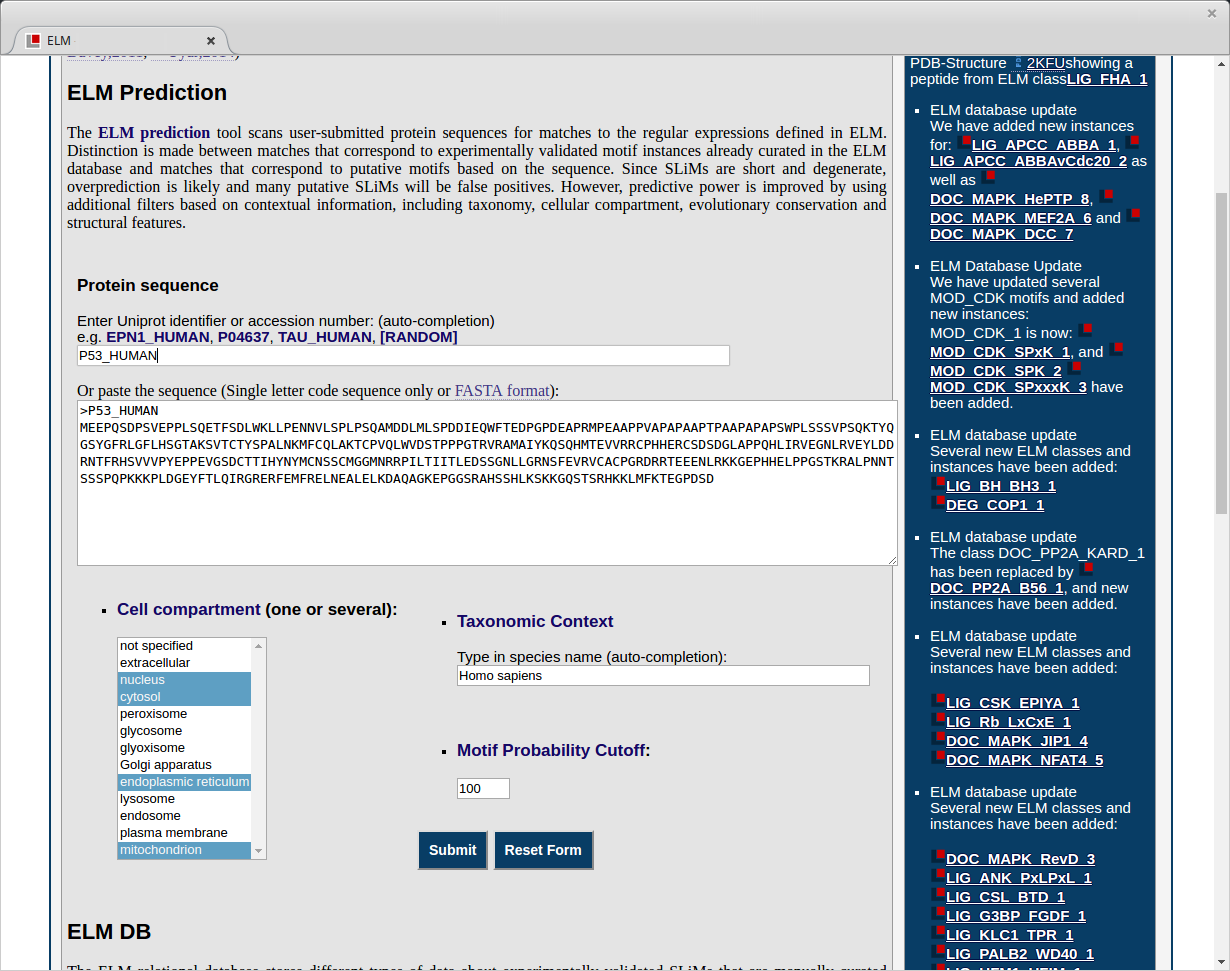
\includegraphics[width=\textwidth]{../Figures/TP53_1/elm_search.png} \textbf{Figure
TP53-BP1-1} The query input page for ELM for predicting motifs in a
given protein sequence.
\end{figure}

Step 1. Open a browser, and navigate to the ELM homepage:
http://elm.eu.org. Enter the Uniprot ID ``P53\_HUMAN'' in the search
field labelled ``Enter a uniprot identifier or accession number''. The
page should autocomplete/suggest the protein ``P53\_HUMAN / P04637 (Homo
sapiens)''. Click on this entry to confirm that we want to search for
SLiM data for this protein. Click on ``Submit'' to view the motif
instance data for p53. (Fig. TP53-BP1-1)

\begin{quote}
The autocompletion mechanism queries uniprot.org for protein identifier;
if it succeeds, then additional information from uniprot will be used to
pre-populate the filter boxes. In this example, P53\_HUMAN is recognized
as a Human protein, and so ``Homo sapiens'' is automatically filled in
the ``Taxonomic Context'' field. Also, P53 has been annotated (by
Uniprot) to be localized to nucleus, cytosol, endoplasmic reticulum and
mitochondrion, so these are also automatically applied as search
criteria. The motif cutoff of ``100'' is a sufficiently high (lenient)
threshold to allow all other detected motifs to be shown.
\end{quote}

step 3. Select the search criteria (optional). It is possible to limit
the results by ``cell compartment'', ``taxonomic context'' or by
changing the ``motif probability cutoff''. To restrict the search to
include SLiM's that are active in certain cellular compartments, select
one or more from the list (use the ``control'' key to select more than
one option). It is also possible to select a ``taxonomic context'' to
restrict the search to SLiMs from certain species. Start typing a
species name in the ``taxonomic context'' input field to get an
auto-completed list of species to select from. Additionaly, a ``Motif
probability cutoff'' can be used to only retain ELM classes whose
pattern probability is below the given value. For the current protocol,
leave all of these at their default values: ``not specified'', ``100''
and no ``taxonomic context''

TODO: Repeat search using stringent filters (homo sapiens, nucleus,
0.01)

\subsection{Interpreting the prediction results: Graphical
Summary}\label{interpreting-the-prediction-results-graphical-summary}

step 4. Click ``submit'' to start the searching for motifs. You will be
brought to an intermediate page indicating that your results are being
processed, and you should be redirected to the final results page within
a minute.

\begin{quote}
The Results are summarized in the first figure on the results page (see
figure TP53-BP1-2). The graphical summary shows the results generated by
the ELM prediction pipeline, combined with additional filters and
information from external resources. The visualization should help you
interpreting the results and to assess whether or not a motif is present
in a sequence, as well as how likely it is to be functional based on its
structural context and evolutionary conservation. Motif instances which
are manually annotated in the database appear as red (TP) or yellow (FP)
ovals in the graphic. Blue/gray squares represent predicted motif
occurrences.

You can bookmark this page: The results are stored for a week.
\end{quote}

\begin{figure}[h!]
\centering
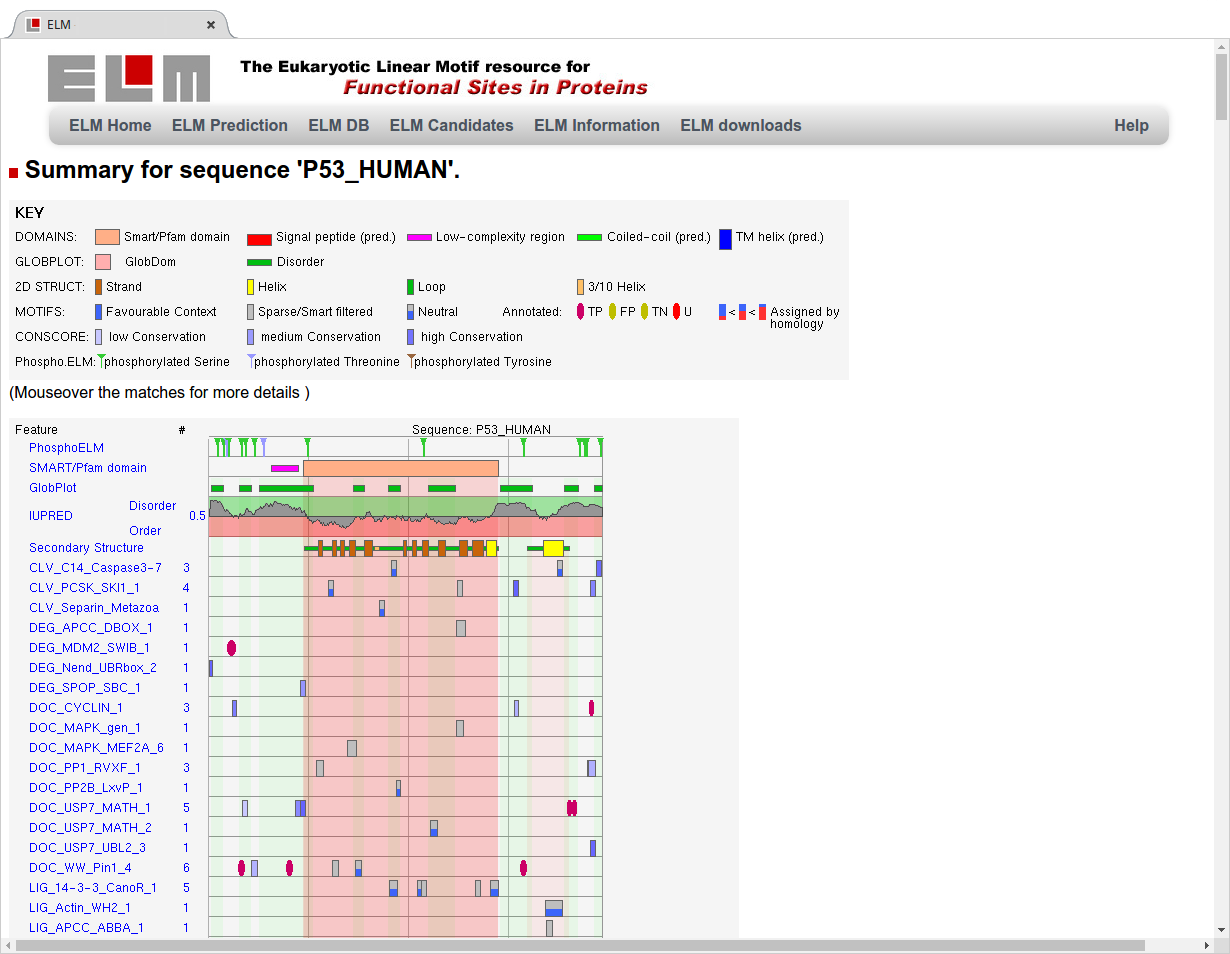
\includegraphics[width=\textwidth]{../Figures/TP53_1/elm_results_summary.png} TODO:
caption
\end{figure}

\textbf{Figure TP53-BP1-2} The graphical results summary of the ELM
Prediction pipeline for ``P53\_HUMAN''. Note that not all motif
detections are shown (the image is truncated at the bottom). The top
five rows show a set of structural features. Annotated and predicted
motifs are shown as differently colored ovals/boxes.

step 6. The first row contains phosphorylation sites as retrieved from
Phospho.ELM (\cite{21062810}), and whether the phosphorylated amino acid
is a serine, threonine or tyrosine. Phospho.ELM is a database of
manually annotated phosphorylation sites obtained from scientific
publications from low and high-throughput experiments. You can follow
the link to Phospho.ELM by clicking on the phosphorylation site in the
image to get more information on individual phosphorylation sites.

\begin{quote}
Phosphorylation sites are only available when the search is performed
with a protein accession (eg. \emph{not} with FASTA sequence alone) in
step XXX and there is relevant information annotated in the Phospho.ELM
database. Phosphorylation sites are relevant to interpret ELM motif
predictions when the predicted motif requires to be phosphorylated (as
in several docking and ligand binding motifs) and naturally, for the
prediction of phosphorylation motifs.
\end{quote}

step 7. The second row shows SMART and Pfam domains detected by the
SMART database (\cite{9600884},\cite{25300481}, \cite{9600884}). Hover
the mouse over these domains to see their names and exact start and end
positions.

\begin{quote}
In order to be functional SLiMs need to be accessble, and therefore they
are usually not found within globular domains and structured regions
(\cite{21909575}). Any SLiMs detected by the ELM prediction pipeline are
less likely to be functional, and are indicated with a red background
(see also the ``structural filter'' described in step XXX).
\end{quote}

step 8. The third row shows globular and disordered regions in the
sequence as predicted by GlobPlot (\cite{12824398}). The fourth and
fifth row contains results from IUPred (\cite{15955779}), another
predictor of disordered protein regions. Protein segments with an IUPred
score above 0.5 considered to be disordered.

\begin{quote}
SLiMs are typically only functional when found in intrinsically
disordered regions. Any motif occurrence detected by the ELM prediction
pipeline that falls within disordered regions are more likely to be
functional.
\end{quote}

step 9. The 5th row contains information on secondary structure. The
secondary structure is predicted using a pipeline mapping motif
occurrence onto high quality reference domain structures
(\cite{19852836}). Check the graphical representation, if the output of
the secondary structure filter and the disorder predictors agree with
respect to wihch parts of the sequence are considered structured and
which disordered.

step 10. The remainder of the figure (below ``secondary structure''
output) displays predicted and annotated motif instances, overlayed by
the structural context from rows 2 and 3 (SMART domains and GlobPlot). A
blue square indicates a single motif occurence, intensity of the color
indicates the conservation of this sequence in homologous proteins.
Boxes in gray are motif occurences which have been filtered out by the
``structure filter''. Boxes that are blue \& gray are neutral (eg.
residing in structural context, but the secondary structure detected a
loop region). If the sequence is already present in the ELM database,
any motif instances that have already been annotated are shown as ovals.
Lastly, any motifs detected, which are annotated to be functional in
homologous sequences, are shown as red/blue rectangles.

TODO: EXPLAIN / SHOW ANNOTATED INSTANCES

\begin{quote}
In the case that not enough homologous sequences were detected to build
an alignment, no conservation score can be calculated. Therefore all of
the motif occurences will be shown in a uniform shade of blue.
\end{quote}

step 11. Place the cursor over the blue box for motif occurence
``MOD\_PLK'' at position 6-12. This motif is in a disordered region, and
has not been filtered out by the structural filter. However, its
conservation score is very low: 0.16, indicating it is not conserved in
homologous proteins.

\begin{quote}
The confidence score is based on how conserved the sequence is across a
set of homolous proteins from other sequences. An full description of
the method can be found in \cite{18460207}.
\end{quote}

step 12. Mouse over a gray rectangle (indicating motifs which have been
filtered out) to find out why this hit was filtered out. It shows scores
for all of the individual criteria used by the secondary structure
filter: The name of the domain, the \emph{accessibility score} ,
\emph{secondary structure score}, \emph{combined total score}, and the
associated \emph{total score P-value} (\cite{19852836}).

\begin{figure}[h!]
\centering
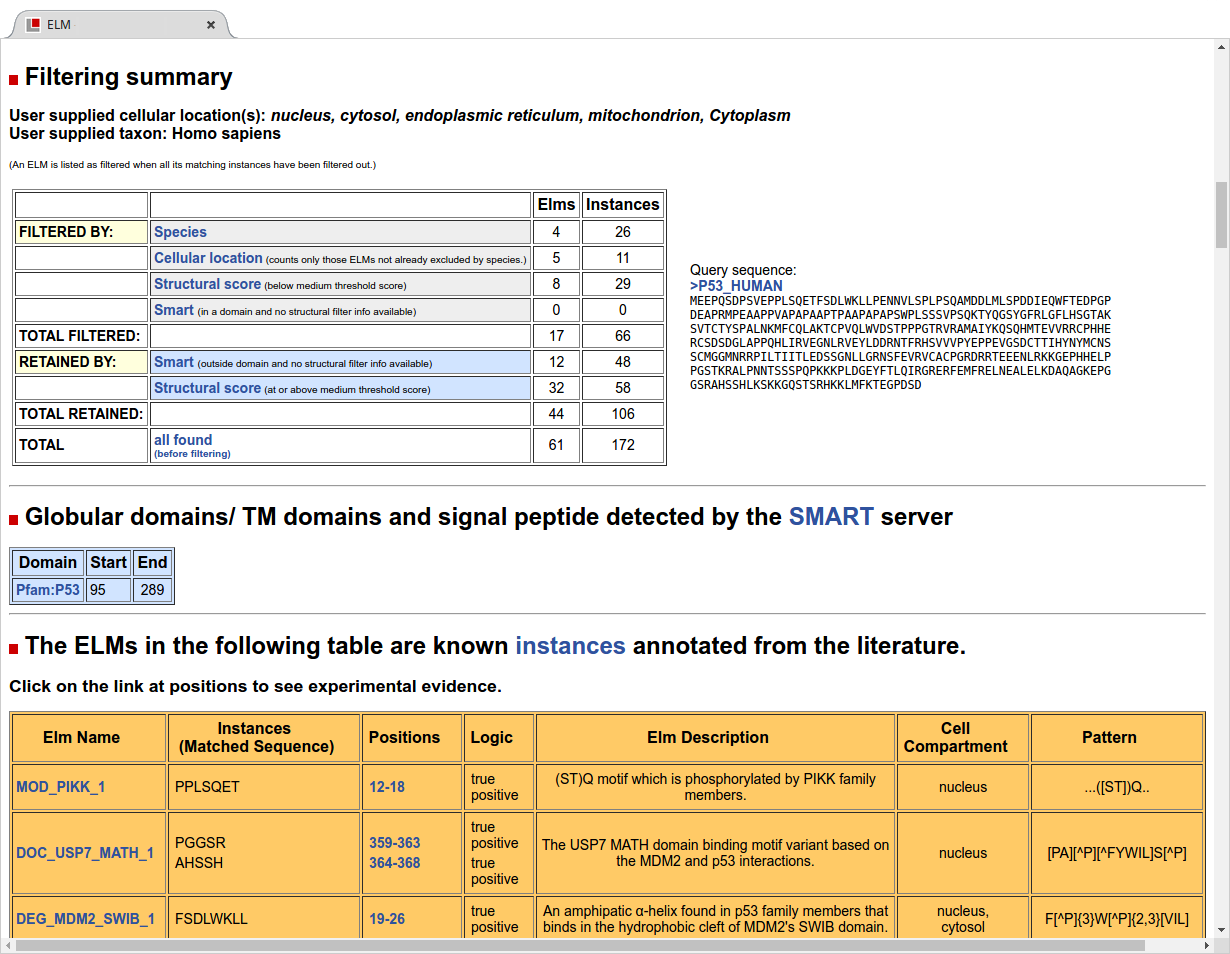
\includegraphics[width=\textwidth]{../Figures/TP53_1/elm_results_alignments_filtering_domains.png}
\textbf{Figure BACT-BP-3:} This section of the results contains
additional details of alignment of homologous proteins, filtering
results and globular domains.

\end{figure}
TODO: INSERT/CHANGE FIGURE/NAME

step 13. Scroll down to below the results graphic to find additional
information on the ELM Predction pipeline's results (figure BACT-BP-3).
The first section contains links to download or view the multiple
sequence alignments of homologous proteins used to calculate the
conservation score. Click on the link ``Click here to enable the
multiple sequence alignment viewer'' to open the alignment in Jalview
(note: this requires the Java browser plugin, which might not be
available on some browsers). Alternatively you can also download the
``alignment'', ``conservation features'' and ``phosphosite features''
files separately to view on a desktop (non-browser) installation of
Jalview (\cite{19151095}).

\begin{quote}
The search for possible homologs is performed against the UniRef90
database, a dataset of protein sequences with less than 90 percent
identity between any two of them (\cite{17379688}). It is also possible
that the BLAST results are not finished when the results page is shown:
We suggest to refresh the page if you see the message ``Either not
enough data available to calculate a sequence alignment or the
calculations haven't finished yet''. In some cases it is also possible
that no homologs will be detected. If you have refreshed the page after
waiting for more than 3 minutes, this is most likely the case.
\end{quote}

step 14. Scroll down to the section titled ``Filtering Summary'' to view
some statistics about how many motifs and instances were filtered out
(figure TP53-BP1-2). The first two lines contain information on whether
and which filters were applied in step XXX of this protocol. The next
two lines (SMART \& Structural score) show how many motifs and instances
were removed by the SMART and Secondary structure filters. The
``Retained by'' section shows how many motif hits were not filtered out
by the ``Smart'' or ``Structural Score'' filter. In this example a total
of XXX instances (of XXX different motifs were identified), of which XXX
instances (and XXX motifs) were filtered out as they occured in a SMART
domain.

\begin{quote}
Note that the graphical summary above does not contain sequences
filtered out by the ``cell compartment'' and ``taxonomic context''
filters (in step XXX). However those filtered out by the SMART and
Structural scores are shown in the graphic above (as gray rectangles).
If any ``cell compartment'' or ``taxonomic context'' filters are
selected in step XXX, the number of motifs and instances are also shown
in this table.
\end{quote}

\begin{figure}[h!]
\centering
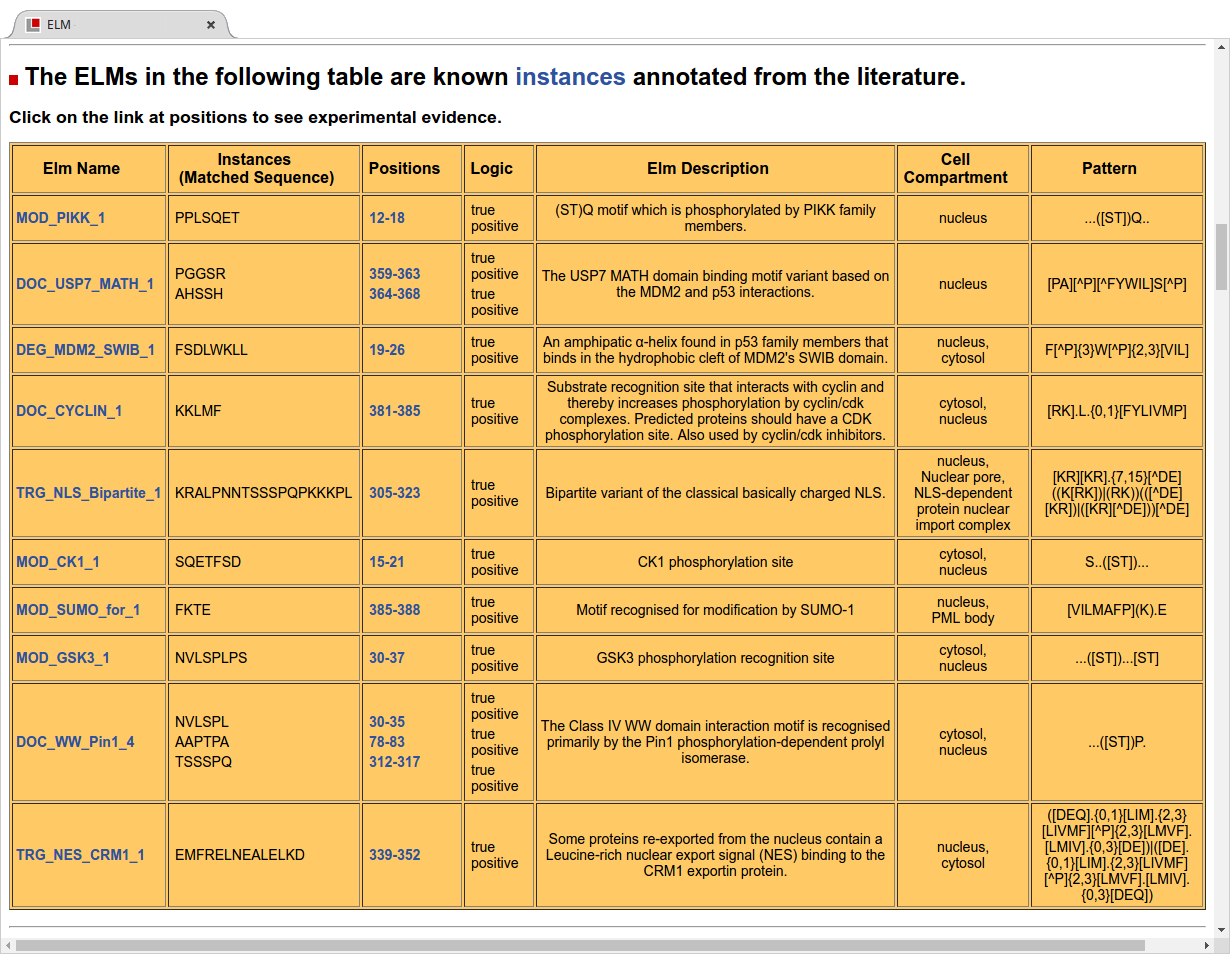
\includegraphics[width=\textwidth]{../Figures/TP53_1/elm_results_known.png} \textbf{Figure
TP53-BP1-3}
\end{figure}

Step 15. On the results page, scroll down to the heading: ``The ELMs in
the following table are known instances annotated from the literature''
(Fig TP53-BP1-3). This table has details of SLiMs which have been
manually annotated in the ELM database. The columns show each motif
name, the sequence(s) that matched the motif as well as their starting
and ending positions and the logic of the annotation followed by a short
description of each motif, to which cell compartments its has been
associated, and finally the regular expression of the motif.

\begin{quote}
The ``Logic'' column indicates whether this motif is an example of a
functional (True Positive, TP) or non-functional (False Positive, FP)
motif. A TP instance is an instance annotated with experimental evidence
showing this instance to be functional, whereas a FP is an instance with
experimental evidence hinting at a function, but after careful
inspection our annotators believe this instance to be non-functional.
There are only rare cases of a true negative (TN) instance, which is an
annotated instance where experiments have shown it to be non-functional.
\end{quote}

TODO: INSERT/CHANGE FIGURE/NAME

step 16. Scroll down to the section with the header ``Globular domains/
TM domains and signal peptide detected by the SMART server'' (Figure
BACT-BP-3). This section contains information on which domains were
detected by the SMART server, and their positions. Clicking on their
names will bring you to the SMART entry for that domain on the SMART
homepage.

TODO: INSERT/CHANGE FIGURE/NAME

\begin{figure}[h!]
\centering
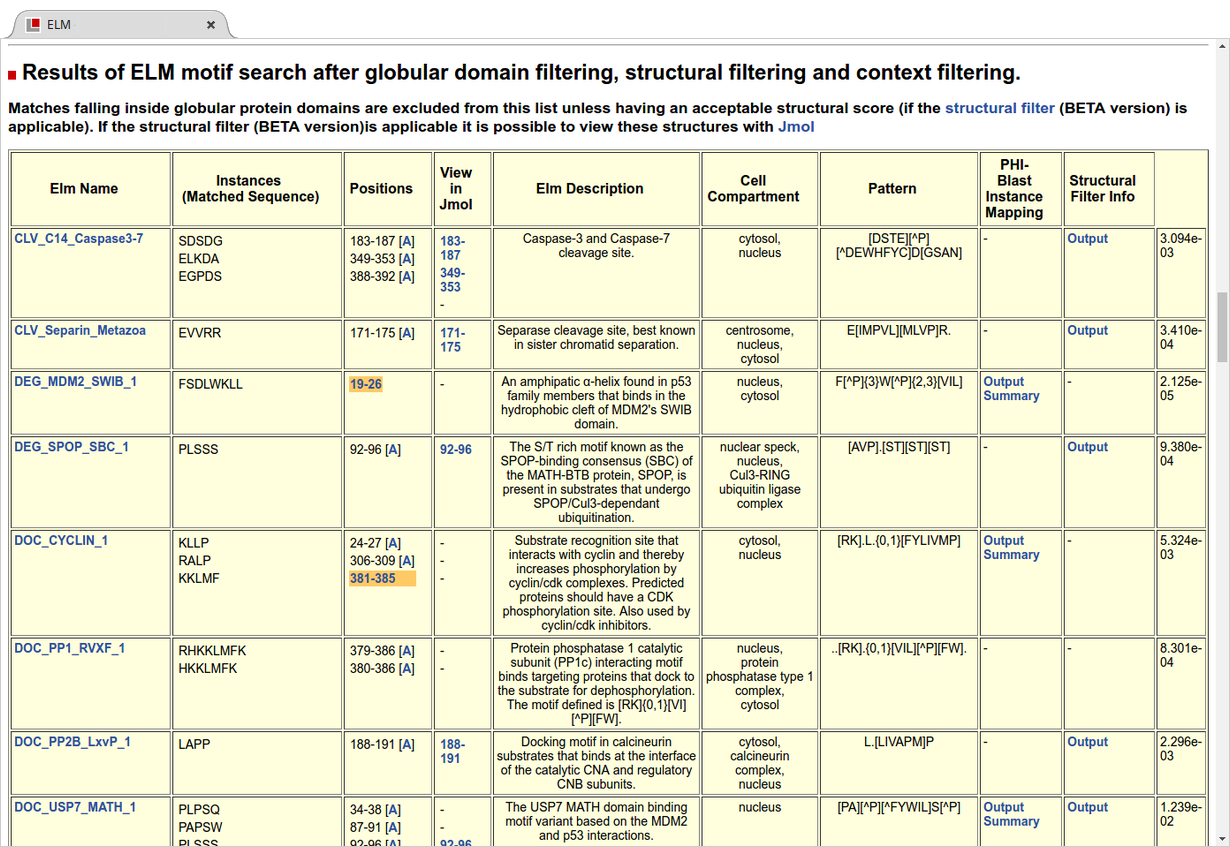
\includegraphics[width=\textwidth]{../Figures/TP53_1/elm_results_motifs.png}
\textbf{Figure BACT-BP-7:} This table contains the list of motifs
detected in the sequence (only the top part of the table is shown).
\end{figure}

TODO: INSERT/CHANGE FIGURE/NAME

step 17. Scroll further down to the section title ``Results of ELM motif
search after globular domain filtering, structural filtering and context
filtering'' to obtain an overview of all of the motifs and motif
instances detected (Figure BACT-BP-7). Each row also contains
information on the Motif name, the matching peptide sequence and its
position. Additional information is shown about the ELM, cell
compartment and its regular expression. If the motif was detected in a
homologue, the column called ``PHI-Blast Instance mapping'' contains
links to the Sequence alignment of the homologous protein, and a summary
of the ELM instance mapper output. If a motif instance has been filtered
out due to Structural criteria (SMART or Structure), this column
contains a link to a page with details on how individual criteria that
make up this filter. The last column contains information on the
Probability filter: the probability reflects the chance to observe this
motif in any random amino acid sequence.

TODO: INSERT/CHANGE FIGURE/NAME

\begin{figure}[h!]
\centering
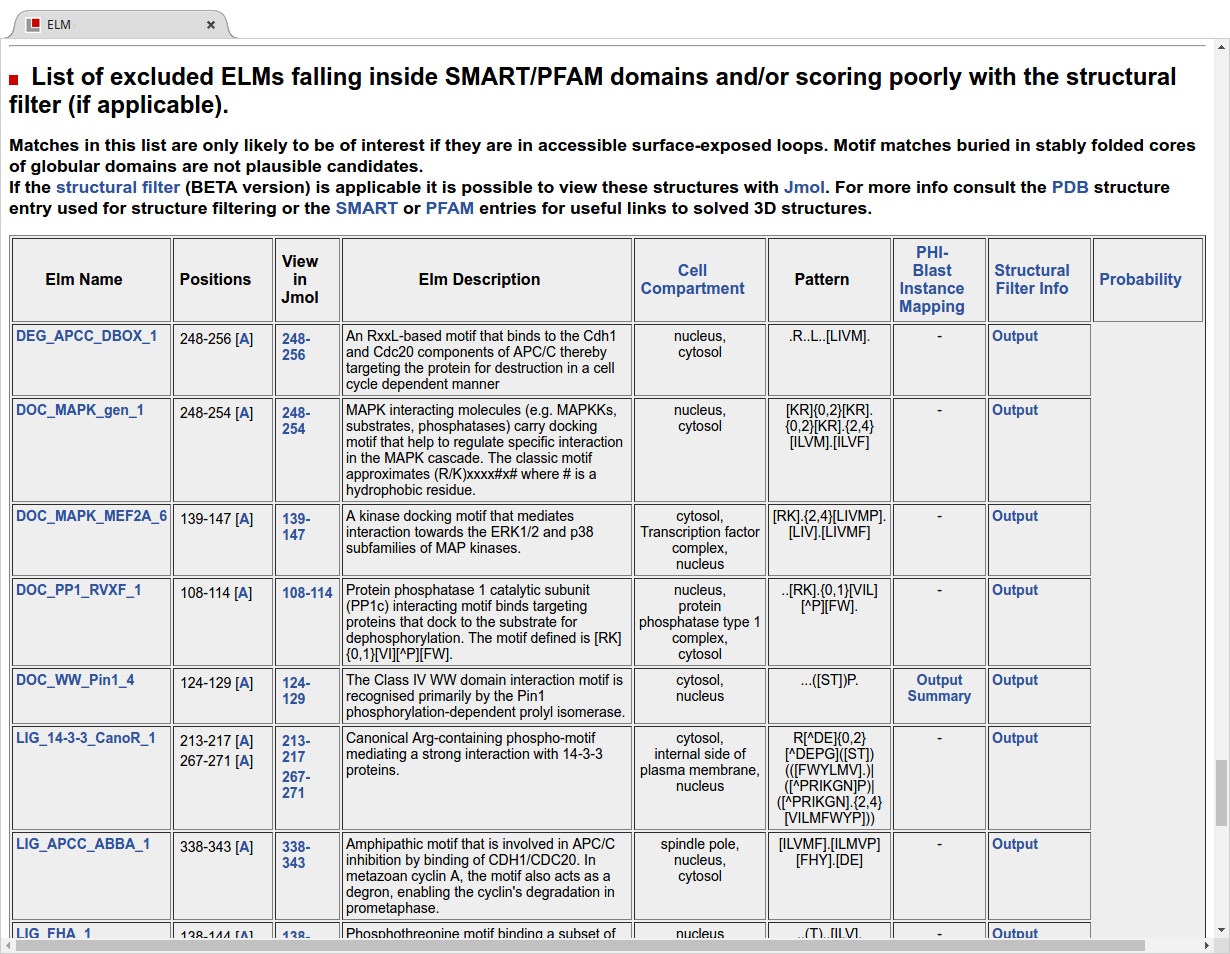
\includegraphics[width=\textwidth]{../Figures/TP53_1/elm_results_motifs_filtered.png}
\textbf{Figure BACT-BP-8:} This table contains the list of motifs
detected in the sequence (only the top part of the table is shown) which
were excluded due to structural filters.
\end{figure}

TODO: INSERT/CHANGE FIGURE/NAME

step 18. Scroll further down to the heading ``List of excluded ELMs
falling inside SMART/PFAM domains and/or scoring poorly with the
structural filter (if applicable).'' (Figure BACT-BP-8). This table is
(almost) identical to the one above, but shows motif instances which
were rejected by the Structural filter or SMART filter.

\section{Alternate Protocol 1: Predicting ELMs in
sequences}\label{alternate-protocol-1-predicting-elms-in-sequences}

TODO: DESCRIBE MOST PROBABLE MOTIF INSTANCES (COMPARED TO FILTERED)

We will use protein ``CV\_0974'' (uniprot ID: Q7NZE8) as an example, a
``probable tyrosine phosphatase'' from \emph{Chromobacterium violaceum}.
This protein is predicted to be a tyrosine phosphates because it has a
``tyrosine phosphatase'' (PTPc) domain.

\subsection{Necessary Resources}\label{necessary-resources-1}

\subsubsection{Software \& Hardware}\label{software-hardware-1}

A modern browser such as Firefox, Chrome, Safari. ELM is best viewed on
a laptop or desktop computer, although tablets and smartphones will also
work.

\subsection{Submitting a query to ELM}\label{submitting-a-query-to-elm}

\begin{figure}[h!]
\centering
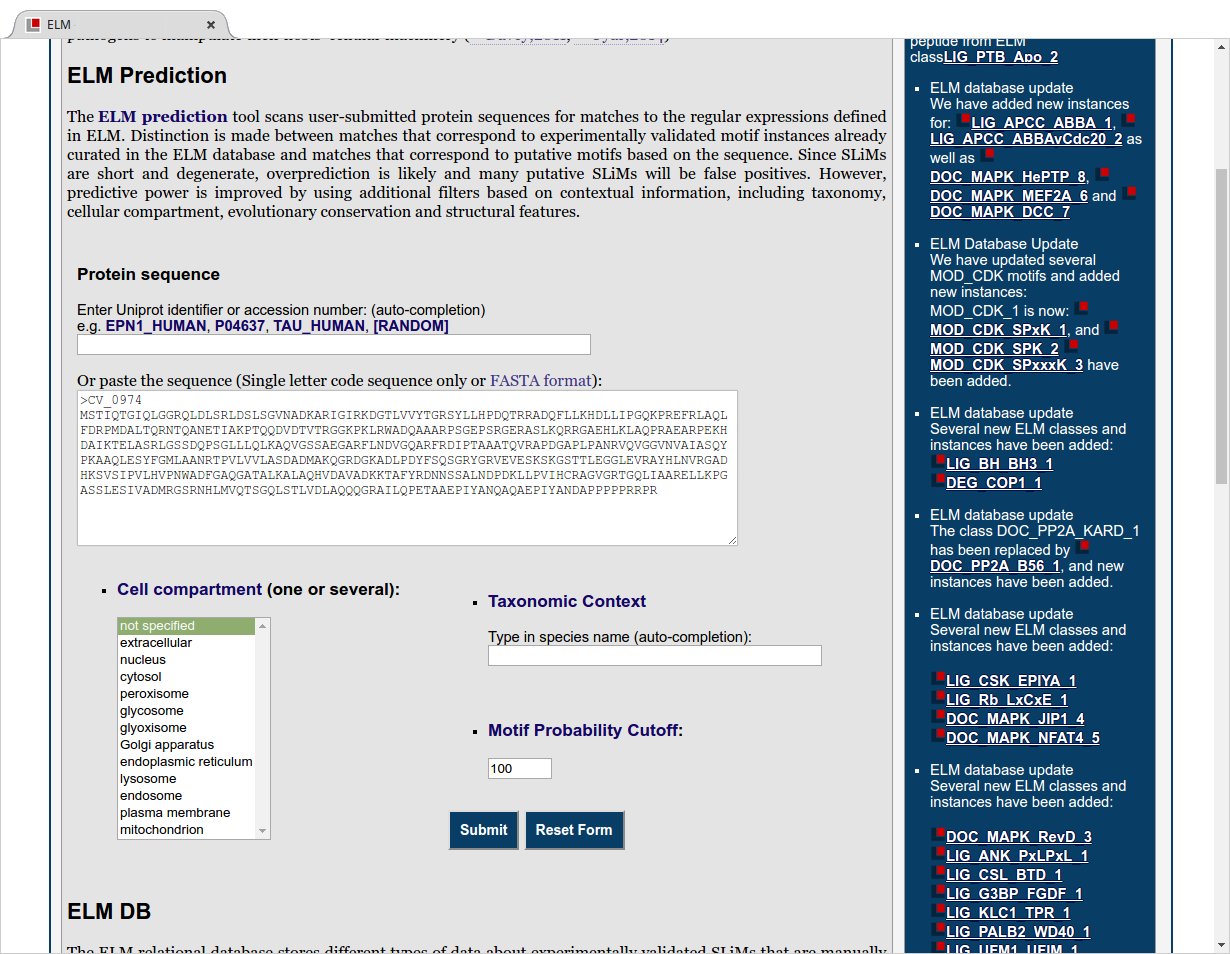
\includegraphics[width=\textwidth]{../Figures/BACT_1/elm_search.png} \textbf{Figure
BACT-BP-1:} The input query page for finding motifs in ELM. The sequence
for \emph{C. vilaceum protein} CV\_0974 was used as an example for this
protocol.
\end{figure}

step 1. Click on the ``ELM Predictions'' button in the menu to access
the search query page (Fig. BACT-BP-1). Here you can provide either a
protein accession (from uniprot) or an amino acid sequence (simply the
sequence, or a FASTA formatted entry) in which you want to detect SLiMs.
Retrieve the FASTA formatted sequence from Uniprot
(http://www.uniprot.org/uniprot/Q7NZE8.fasta), and enter it into the
``sequence input text box''.

TODO: MENTION NOT TO USE ``CHROMOBACTERIUM VIOLACEUM'' IN THE ORGANISM
BOX AND WHY

\begin{figure}[h!]
\centering
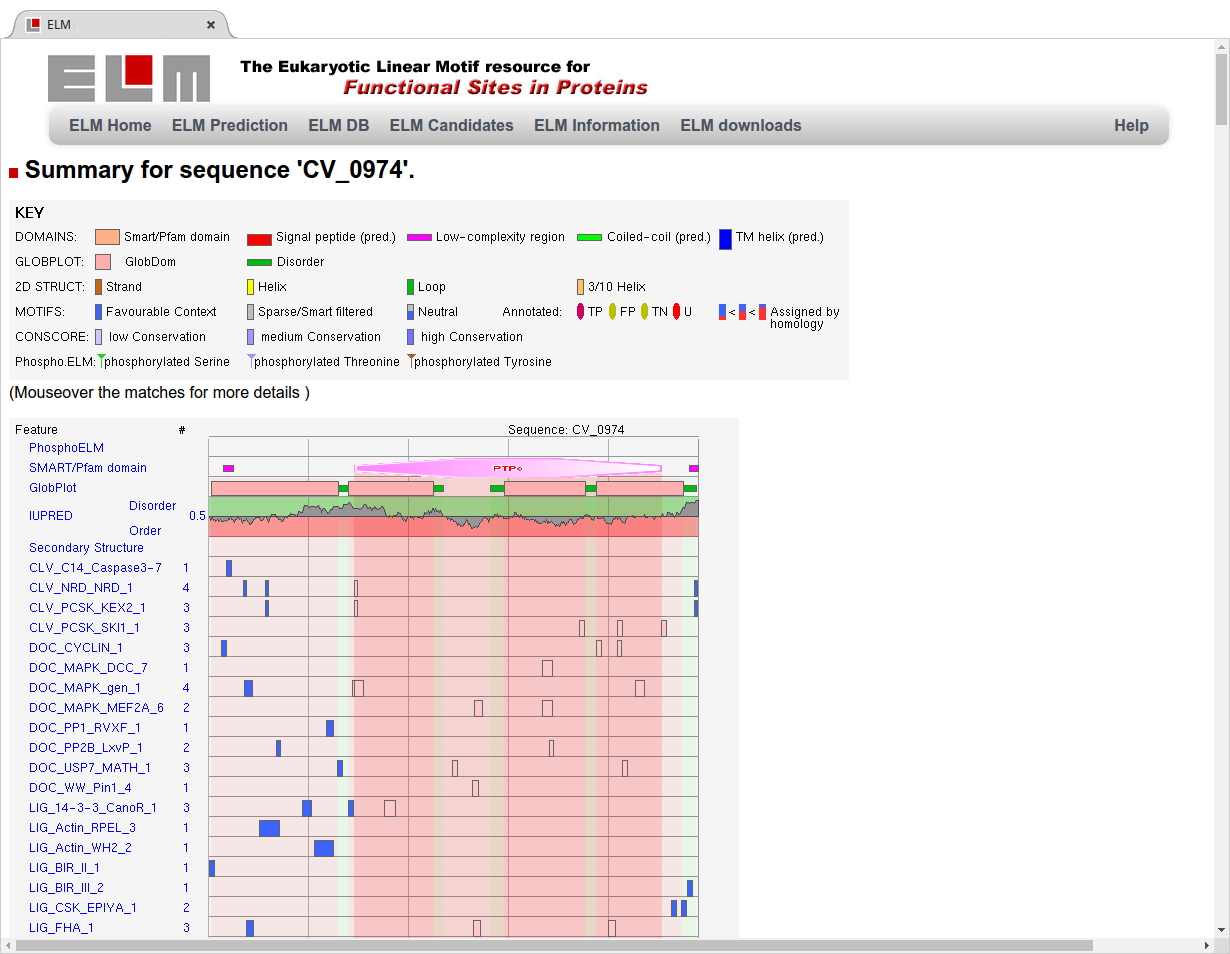
\includegraphics[width=\textwidth]{../Figures/BACT_1/elm_results_summary.png}
\textbf{Figure BACT-BP-2:} The graphical results summary of the ELM
Prediction pipeline for Probable Tyrosine phosphate (CV\_0974). Note
that not all motif detections are shown (the image is truncated at the
bottom). The top five rows show a handfull of structural features. The
motif occurence are shown as blue boxes, the intensity of which
indicates the conservation score. See steps XXX to YYY for more
information.
\end{figure}

step 2. The Results are summarized in the first figure on the results
page (see figure BACT-BP-2). The Graphical summary shows all of the
final and intermediate results generated by the ELM Prediction pipeline,
and can be used infer whether or not a motif is present in a sequence,
as well as now likely it is to be functional based on its structural
context and evolutionary conservation.

step 3. Check the first row to see whether there are for phosphorylation
sites acid is a serine, threonine or tyrosine. In this case, no
phosphorylation data could be found in the Phospho.ELM database
(\cite{21062810}).

step 4. Check the second row showing SMART and Pfam domains. Hover the
mouse over these domains to see their names and exact start and end
positions.

step 5. The third row shows globular and disordered regions in the
sequence as predicted by GlobPlot (\cite{12824398}). The 4th \& 5th rows
contain results from IUPred (\cite{15955779}), another unstructured
region prediction tool. Protein segments with an IUpred score above 0.5
are 95\% likely to be disorered (REF???).

step 6. Place the cursor over the blue box for motif occurence
``DOC\_USP7\_MATH\_1'' at position 129-133. This motif is in a disorered
region, and has not been filtered out by the structural filter. However,
its conservation score is extremely low: 0.000, indicating it is not
conserved in homologous proteins. Place the cursor over motif
``DOC\_MAPK\_DCC\_7'' at positions ``334-343''. Despite the high
conservation score (1.000), this motif is inside the PTPc domain (and a
Globular regions), and therefore has been filtered out.

TODO: CHECK CONSERVATION FILTER

\subsection{Interpreting the prediction results: Additional
Information}\label{interpreting-the-prediction-results-additional-information}

TODO: DESCRIBE HOW TO INTERPRETE THE PREDICTIONS USING THIS BACTERIAL
EXAMPLE (OF WHICH NOT MUCH IS KNOWN). FOCUS ON HOW ONE SHOULD INTERPRETE
THESE PREDICTIONS (LOOK AT DISORDER/GLOBULARITY, CONSERVATION)

\section{Alternate Protocol 4: Predicting ELMS in sequences using REST
API}\label{alternate-protocol-4-predicting-elms-in-sequences-using-rest-api}

Querying ELM for motifs in a given sequence (as discussed in basic
protocol 1), gives you a nice overview of putative and possibly
annotated motifs in your query protein with a graphical representation
using colors to highlight different regions of the protein sequence (eg.
disordered vs.~globular). It is however difficult to analyse a large set
of protein sequences in this manner. Therefore, http://elm.eu.org
provides an interface which you can use to submit your sequence in a
programmatic way. Of course, this way, you won't receive the graphical
output representation, but are limited to textual data representation.

Currently, there exists a single URL `http://elm.eu.org/start\_search/'
to accept such queries. You can choose to either submit a uniprot name
or accession (ex. `http://elm.eu.org/start\_search/P53\_HUMAN.tsv') or
submit your raw sequence (ex.
`http://elm.eu.org/start\_search/MAPRGFSCLLLLTSEIDLPVKRRA').

The logic here is, if the URL ends in `.tsv' then the server assumes you
are using a Uniprot id or accession; if it doesn't, then it assumes you
are using raw sequence. See below for details.

\subsection{Necessary Resources}\label{necessary-resources-2}

\subsubsection{Software}\label{software}

Ideally use \texttt{curl} https://curl.haxx.se/ on the command line.
This program can be launched from the terminal in any of the major
operating systems: OSX, Windows and Linux. Of course \texttt{curl} is
only one of many different ways to access web content programatically,
and we suggest anyone to use which ever program they feel is better
suited for their tasks.

\subsection{Submitting a query to ELM via
REST}\label{submitting-a-query-to-elm-via-rest}

step 1. Use \texttt{curl} to query ELM for all motifs predicted to occur
in Human P53 by typing the following into a terminal: `curl
`http://elm.eu.org/start\_search/P53\_HUMAN.tsv'. Each row represents a
motif detection, and the first column ``elm\_identifier'' indicates
which class was identified. The columns ``start'' and ``stop'' show that
first and last amino acid positions that matched form part of the motif.
``is annotated'' is True if this motif has been annotated in the
database as an (experimentally validate) motif instance. ``is
phiblastmatch'' is True if ?????. The column ``is filtered'' shows
whether or not this motif was rejected by the ELM Prediction structure
filter. ``phibast'' indicates whether ?????. The ``topodomfilter'' and
``taxonfilter'' shown whether ?????. The last column ``structure'' ?????

\begin{quote}
In Figure \emph{ELM predictions pP53} we used a sligtly more advanced
command to get the output to look nice in the terminal. We specified the
\texttt{-s} option to silence all \texttt{curl} output other than the
downloaded file, and piped (\texttt{\textbar{}}) the output directly to
the \texttt{column} command (this command exists on most Linux and OSX
machines).
\end{quote}

TODO: REDO FIGURE as it shows browser in transparent background

\begin{figure}[h!]
\centering
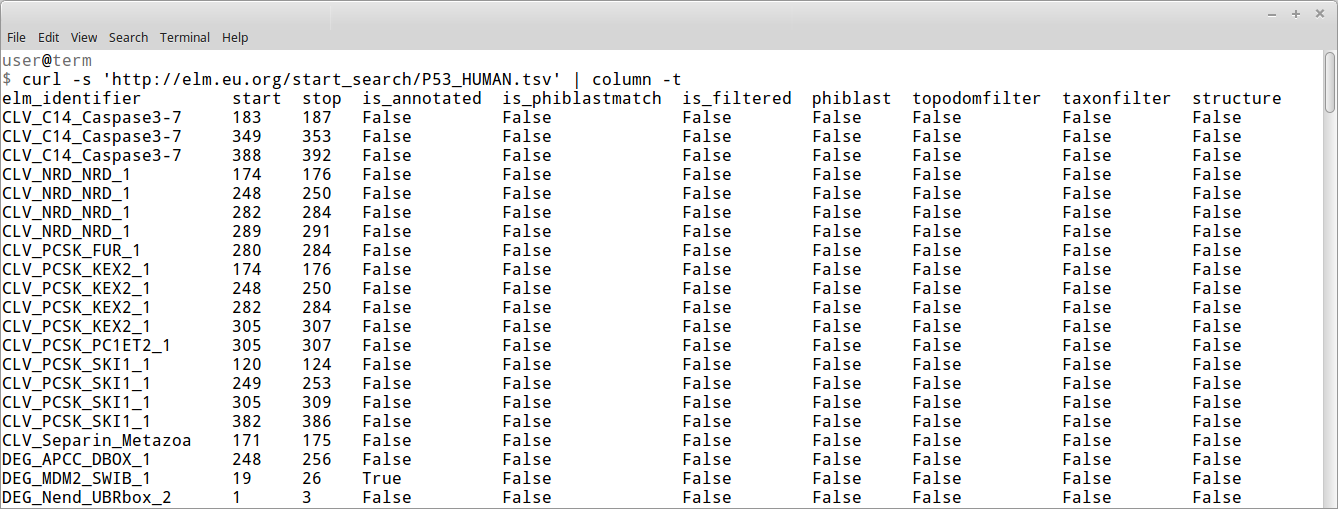
\includegraphics[width=\textwidth]{../Figures/BACT_3/curl_P53.png} \textbf{Figure ELM
Predictions P53:} The commandline output when \texttt{curl} is used to
donload all motifs predicted in Human P53. Note that we used a more
advanced command that \texttt{curl} alone to make the columns align
nicely (see text for an explanation).

\end{figure}

step 2. Use \texttt{curl} to query ELM via protein sequence by using the
URL `http://elm.eu.org/start\_search/MAPRGFSCLLLLTSEIDLPVKRRA' (Figure
BACT-AP3-query). In this case the the query is an arbitrary short
peptide sequence, but this can (of course) contain any sequence you are
intersted in analysing. The output format is exactly the same as in the
previous step.

\begin{quote}
This way of querying ELM is unfornataly not stable for long protein
sequences. Different browsers and computers have different maximum
lengths for URLs, and the excess text is often simply ignored. We
reccomend not using this method for sequences longer than 2000 amino
acids.
\end{quote}

TODO: REDO FIGURE as it shows browser in transparent background

\begin{figure}[h!]
\centering
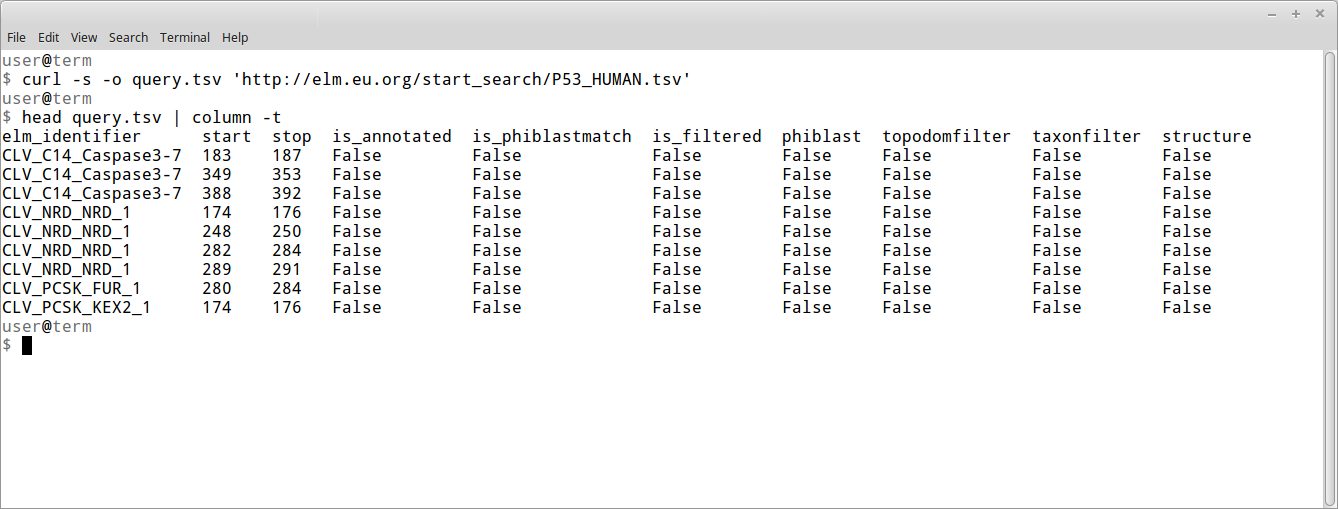
\includegraphics[width=\textwidth]{../Figures/BACT_3/predictions_query.png} \textbf{Figure
ELM Predictions on query sequence:} It is also possible to send amino
acid sequences to the ELM Prediction pipeline. In this case we have used
the curl option \texttt{-o} to download directly to the file
\texttt{query.tsv}, and use a combination of the \texttt{head} and
\texttt{column} commands to display the first 10 rows to the terminal.

\end{figure}
TODO: add this information to the download page

TODO: maybe rename \texttt{start\_search} to \texttt{query}?

\section{Alternate Protocol 3: Searching the ELM database using REST
API}\label{alternate-protocol-3-searching-the-elm-database-using-rest-api}

Many researchers are interested in large-scale analyses rather than
information about individual protein sequences. To this end, individual
queries to the ELM webserver with a single protein id at a time, are not
practical.

For this reason, as much information as possible is made available via a
REST interface (\cite{Fielding_2002}). This allows the user to interact
with the ELM database and ELM webserver via scriptable URL requests.
Each request can easily be tested in the browser before it is being
automated in a script.

In this section we will explore the various ways in which data can
downloaded both in using the browser as well as via the commandline.

\subsection{Necessary Resources}\label{necessary-resources-3}

\subsubsection{Software}\label{software-1}

Ideally use \texttt{curl} https://curl.haxx.se/ on the commandline. This
program can be launched from the terminal in any of the major operating
systems: OSX, Windows and Linux. Of course \texttt{curl} is only one of
many different ways to access web content programatically, and we
suggest anyone to use which ever program they feel is better suited for
their tasks.

\subsection{Downloading all ELM
classes}\label{downloading-all-elm-classes}

\begin{figure}[htbp]
\centering
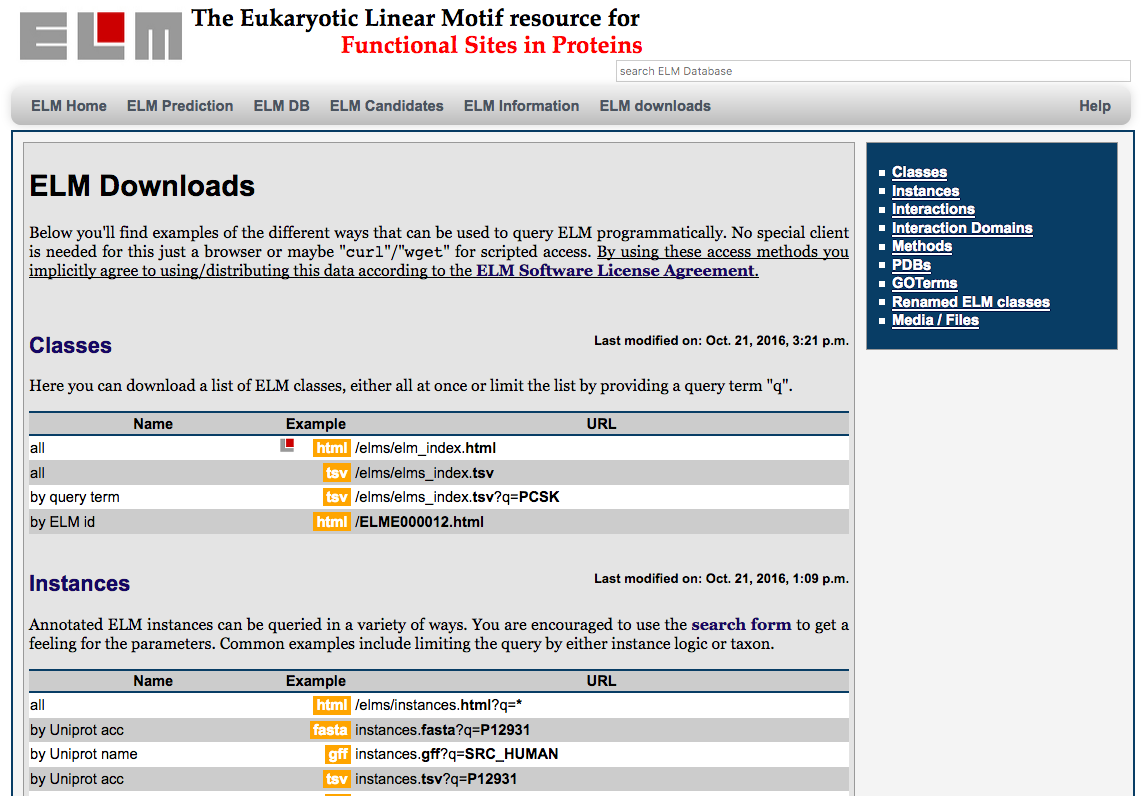
\includegraphics[width=\textwidth]{../Figures/BACT_2/elm_downloads_html.png}
\end{figure}

\textbf{Figure ELM-Downloads:} The ELM downloads page, which holds
information about the different types of data (such as ``Classes'',
``Instances'', etc; see menu to the right) that can be obtained from the
server. The orange boxes are clickable links, the URL following them are
used to highlight the URL scheme used by the server (bold font denotes
specifics used in the examples such as query terms, or formats).

step 1. Direct your browser to the URL `http://elm.eu.org/downloads' or
select `ELM Downloads' from the main Menu (Figure ELM-Downloads) This
webpage contains links and descriptions on how to download ELM data in
text format. The datasets are split into several smaller collections
(for example ``Classes'', ``Instances'', etc). Each table contains links
(in orange) to download the data in various formats.

\begin{quote}
Each table also shows the `last modified date' indicating when the data
was last updated. This is useful if you want to know when to update your
local data with the most up to date ELM data.
\end{quote}

step 2. Click on the first orange `html' link in the table ``Classes''
to navigate to the following URL:
`http://elm.eu.org/elms/elm\_index.html'. This page shows all of the
annotated ELM classes in the database. This page is the same one as
shown in Figure \emph{TP53-BP1-classses}

step 3. Navidate to the folling URL:
`http://elm.eu.org/elms.html?q=CSK', specifying ``q=CSK'' to limit the
list of ELMs to those matching the search query ``CSK''. This page is
again similar to the one shown in Figure \emph{TP53-BP1-classses}, but
with less classes.

\begin{quote}
This search result is identical to the result you would obtain by doing
a ``manual'' search on the ELM Classes page
(http://elm.eu.org/elms.html). The column descriptions are also the same
as described in Step XXX in Protocol YYY.
\end{quote}

\begin{figure}[h!]
\centering
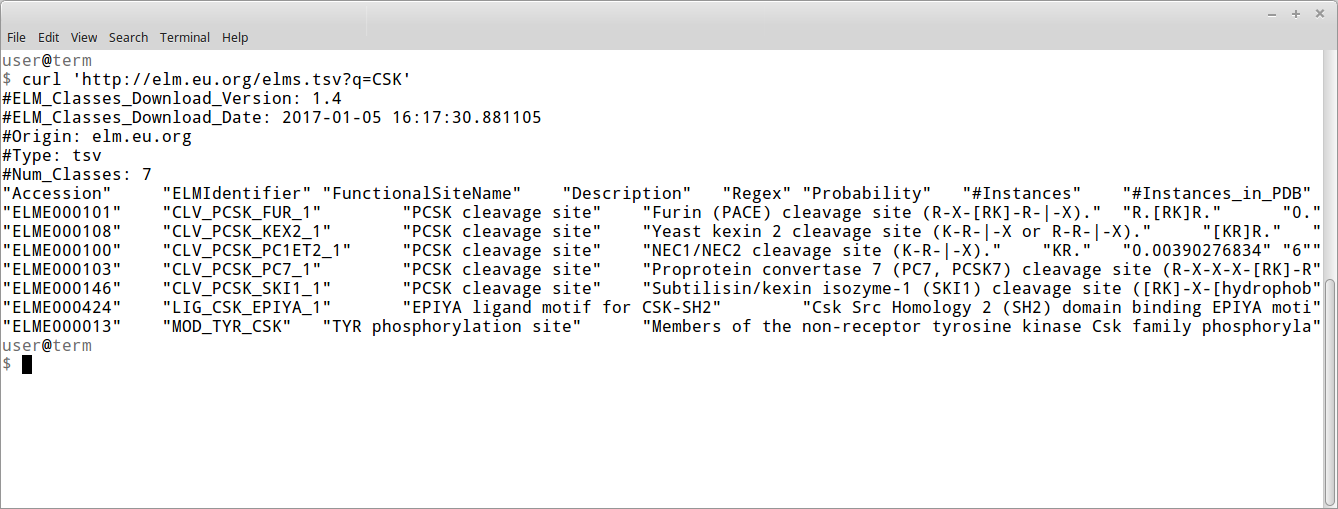
\includegraphics[width=\textwidth]{../Figures/BACT_2/elm_curl_classes_CSK.png}
\textbf{Figure ELM-Curl-Classes}: Screenshot of a terminal window using
\texttt{curl} to download all ELM classes matching the term `CSK'.

\end{figure}

step 4. Open the following URL: `http://elm.eu.org/elms.tsv?q=CSK' to
download a list of classes that match the search query ``CSK'' (as in
the previous step) in the ``tab separated values'' format. By exchanging
the `.html' part of the url with `.tsv', we ask the webserver to give us
the data in TSV (tab-separated values) format.

\begin{quote}
Depending on which browser you are using, the file may open directly in
your browser, or you may be prompted to download the file or save it to
a separate location. In the latter two cases you can open the downloaded
file using a (plain) text file viewer, or possible a spreadsheet viewer
(such as Microsoft Excel).
\end{quote}

step 5. Type the follwing command into a command line terminal to
download the same data from the previous step directly into the
terminal: \texttt{curl 'http://elm.eu.org/elms/elms\_index.tsv?q=CSK'}.
The output should look similar to \emph{Figure ELM-Curl-Classes}. The
column names are still the same ones as shown in the \emph{classes}
table in Figure \emph{BACT-AP2-Elm-classes-downloads}.

\begin{quote}
Use the curl option \texttt{-o} to save the results directly to a file.
For example:
\texttt{curl -o classes.tsv 'http://elm.eu.org/elms/elms\_index.tsv?q=CSK'}
will save the data to a file called \emph{classes.tsv}.
\end{quote}

step 6: To download a list of all motif instances detected in Human P53,
type the followin command into a terminal:
\texttt{curl 'http://elm.eu.org/instances.gff?q=p53\_human'}. The output
should look similar to that shown in figure \emph{Figure ELM-Curl-P53}.
The output is in the ``General Feature Format''
(http://www.ensembl.org/info/website/upload/gff.html\#moreinfo), with
the FASTA formatted sequence appended to the end of the output.

\begin{quote}
Many other file formats are available for downloading instances
annotations, including the FASTA, GFF, PIR, or PSI-MI format (either XML
or MiTab) {[}24067240{]}.
\end{quote}

\begin{figure}[h!]
\centering
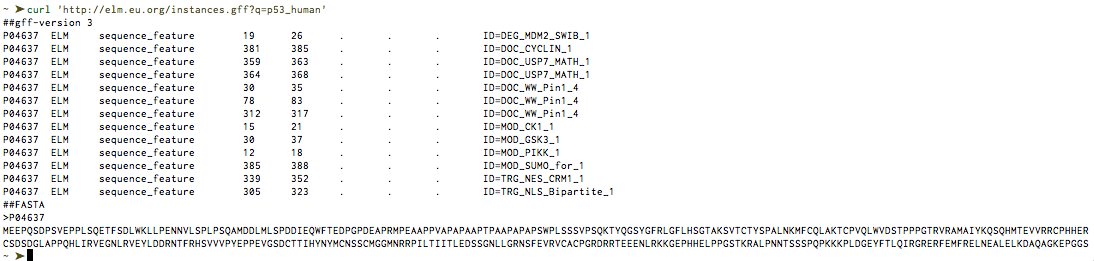
\includegraphics[width=\textwidth]{../Figures/BACT_2/elm_curl_instances_p53_human.png}
\textbf{Figure ELM-Curl-Instances-P53}: Screenshot of a terminal window
using \texttt{curl} to download all ELM instances annotated for sequence
p53\_human.
\end{figure}

step 7. To download a list of all instances matchin th search query
``CLV'' in the yellow fever mosquito (Aedes agypti), enter the following
command into a terminal: `curl
`http://elm.eu.org/instances.tsv?q=CLV\&taxon=aedes+aegypti'. In general
any species name can be used, always replacing the ``space'' with a
``+''. This should return a single instance, the only one matching CLV
in A. aegypti.

step 8. More data (interactions, domains, methods, etc.) can be
downloaded from ELM in analogous fashion as shown in the preceeding
steps. Take a look at the ELM Downloads page
(http://elm.eu.org/downloads, Figure \emph{BACT-AP2-Elm-downloads}) for
an overview of which datasets can be downloaded, and what the different
possible filters and formats are for each dataset.

\% NOTE: TODO: Mention ELM software license agreement?

\section{Guidelines for Interpreting
Results}\label{guidelines-for-interpreting-results}

\emph{instructions: A brief discussion of the theory and applications of
your}

\emph{notes: Maybe mention how findings are relevant to the lab? For
example: Manually annotated content should be reliable, although one
should look at the `confidence' in the instance annotation. Predictions
are probably trustworthy, but you need to take into account the
`confidence score', and other features like whether its in a domain,
etc\ldots{}}

\section{Commentary:}\label{commentary}

\emph{instructions: A brief discussion of the theory and applications of
your}

\subsection{Background Information}\label{background-information}

\textbf{Im still not sure what's going to happen here :(}

In order to interpret the data contained in ELM and the results produced
by the ELM prediction tool, it is important to have a basic
understanding of SLiM's and how they are affected by their structural
and biological context.

Taking into account additional information, besides a match to a
sequence pattern defining a SLiM, can greatly narrow the selection of
putative motifs for experimental validation.

SLiM's operate via with interactions with other proteins, typically the
surface of a globular, domain in a protein, although some are known to
bind to disordered regions. As their name suggests, SLiMs are compact,
being composed of a limited number of adjacent amino acids. Most of a
motif's binding specificity however is conferred by only a subset of
these amino acids. Those few residues that directly interact with the
binding partner are evolutionary conserved, although in many cases a
subset of amino acids that share certain properties (such as similar
charge, size or hydrophobicity) are allowed in these hotspot positions.
In the motif positions that contribute little to the interaction, there
are even less constraints, i.e.~a broader range of amino acids is
allowed in these positions (\cite{21909575}). A first consequence of
this degeneracy is that SLiMs co-operatively engage in interactions of
relatively low affinity. Hence these binding events are transient and
reversible, and can be readily modulated, for instance by PTM.

\begin{figure}[h!]
\centering
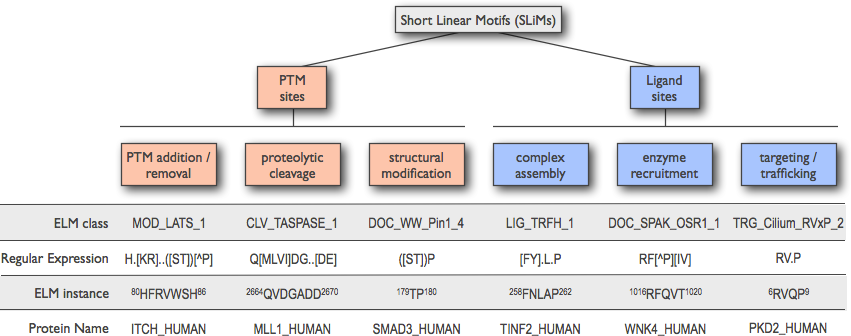
\includegraphics[width=\textwidth]{../Figures/functional_classification_of_SLiMs.png}
\textbf{Figure functional\_classification\_of\_SLiMs} For each ELM
class, the functional category to which it belongs is indicated by a
three-letter prefix. Each ELM class is defined by a regular expression.
Peptide sequences in proteins that match the regular expression of a
specific ELM class and that were experimentally validated to be
functional motifs are captured as ELM instances of that class. Degrons
are a specific subtype of enzyme-recruiting docking motifs (see text for
a detailed description).
\end{figure}

\subsection{Critical Parameters and
Troubleshooting}\label{critical-parameters-and-troubleshooting}

\emph{instructions: optionally 2 separate sections.}

\section{Internet Resources with
Annotations}\label{internet-resources-with-annotations}

http://www.clustal.org/omega Clustal Omega (\cite{21988835}) is a tool
for the alignment of multiple nucleic acid and protein sequences.

http://www.jalview.org Jalview (\cite{19151095}) is a Java desktop
application (and browser applet) that employs web services for sequence
alignment and visualization.

http://proviz.ucd.ie ProViz (\cite{27085803}) is an interactive protein
exploration tool, which searches several databases for information about
a given query protein. Data relevant to the protein like an alignment of
homologues, linear motifs, post translational modifications, domains,
secondary structure, sequence variations and others are graphically
represented relative to their position in the protein.
